\documentclass[10]{article}
%\documentclass[11pt]{book}
\usepackage{hyperref}
\usepackage{amsfonts,amssymb,amsmath,amsthm,cite}
\usepackage{graphicx}
\usepackage[toc,page]{appendix}
\usepackage{nicefrac}
%% \usepackage[francais]{babel}
\usepackage[applemac]{inputenc}
\usepackage{amssymb, euscript}
\usepackage[matrix,arrow,curve]{xy}
\usepackage{graphicx}
\usepackage{tabularx}
\usepackage{float}
\usepackage{tikz}
\usepackage{slashed}
\usepackage{mathrsfs}
\usepackage{multirow}

%\usepackage{mathtools}

\usetikzlibrary{matrix}

\usepackage[T1]{fontenc}
\usepackage{amsfonts,cite}
\usepackage{graphicx}

%% \usepackage[francais]{babel}
\usepackage[applemac]{inputenc}


\usepackage[sc]{mathpazo}
\usepackage{environ}

\linespread{1.05}         % Palatino needs more leading (space between lines)


%\usepackage[usenames]{color}



\DeclareFontFamily{T1}{pzc}{}
\DeclareFontShape{T1}{pzc}{m}{it}{1.8 <-> pzcmi8t}{}
\DeclareMathAlphabet{\mathpzc}{T1}{pzc}{m}{it}
% the command for it is \mathpzc

\textwidth=140mm


% % % % % % % % % % % % % % % % % % % %
\theoremstyle{plain}
\newtheorem{prop}{Proposition}[section]
\newtheorem{prdf}[prop]{Proposition and Definition}
\newtheorem{lem}[prop]{Lemma}%[section]
\newtheorem{cor}[prop]{Corollary}%[section]
\newtheorem{thm}[prop]{Theorem}%[section]
\newtheorem{theorem}[prop]{Theorem}
\newtheorem{lemma}[prop]{Lemma}
\newtheorem{proposition}[prop]{Proposition}
\newtheorem{corollary}[prop]{Corollary}
\newtheorem{statement}[prop]{Statement}

\theoremstyle{definition}
\newtheorem{defn}[prop]{Definition}%[section]
\newtheorem{cordefn}[prop]{Corollary and Definition}%[section]
\newtheorem{empt}[prop]{}%[section]
\newtheorem{exm}[prop]{Example}%[section]
\newtheorem{rem}[prop]{Remark}%[section]
\newtheorem{prob}[prop]{Problem}
\newtheorem{conj}{Conjecture}       %% Hypothesis 1
\newtheorem{cond}{Condition}        %% Condition 1
%\newtheorem{axiom}[thm]{Axiom}           %% Axiom 1 modified
\newtheorem{fact}[prop]{Fact}
\newtheorem{ques}{Question}         %% Question 1
\newtheorem{answ}{Answer}           %% Answer 1
\newtheorem{notn}{Notation}        %% Notations are not numbered

\theoremstyle{definition}
\newtheorem{notation}[prop]{Notation}
\newtheorem{definition}[prop]{Definition}
\newtheorem{example}[prop]{Example}
\newtheorem{exercise}[prop]{Exercise}
\newtheorem{conclusion}[prop]{Conclusion}
\newtheorem{conjecture}[prop]{Conjecture}
\newtheorem{criterion}[prop]{Criterion}
\newtheorem{summary}[prop]{Summary}
\newtheorem{axiom}[prop]{Axiom}
\newtheorem{problem}[prop]{Problem}
%\theoremstyle{remark}
\newtheorem{remark}[prop]{Remark}

\numberwithin{equation}{section}
\newtheorem*{claim}{Claim}
\DeclareMathOperator{\Dom}{Dom}              %% domain of an operator
\newcommand{\Dslash}{{D\mkern-11.5mu/\,}}    %% Dirac operator


%\newcommand\myeq{\stackrel{\mathclap{\normalfont\mbox{def}}}{=}}
\newcommand{\nor}[1]{\left\Vert #1\right\Vert}    %\nor{x}=||x||
\newcommand{\vertiii}[1]{{\left\vert\kern-0.25ex\left\vert\kern-0.25ex\left\vert #1
		\right\vert\kern-0.25ex\right\vert\kern-0.25ex\right\vert}}
\newcommand{\Ga}{\Gamma}  
\newcommand{\coker}{\mathrm{coker}}                   %% short for  \Gamma
\newcommand{\Coo}{C^\infty}                  %% smooth functions
% % % % % % % % % % % % % % % % % % % %


\usepackage[sc]{mathpazo}
\linespread{1.05}         % Palatino needs more leading (space between lines)

\newbox\ncintdbox \newbox\ncinttbox %% noncommutative integral symbols
\setbox0=\hbox{$-$} \setbox2=\hbox{$\displaystyle\int$}
\setbox\ncintdbox=\hbox{\rlap{\hbox
		to \wd2{\hskip-.125em \box2\relax\hfil}}\box0\kern.1em}
\setbox0=\hbox{$\vcenter{\hrule width 4pt}$}
\setbox2=\hbox{$\textstyle\int$} \setbox\ncinttbox=\hbox{\rlap{\hbox
		to \wd2{\hskip-.175em \box2\relax\hfil}}\box0\kern.1em}

\newcommand{\ncint}{\mathop{\mathchoice{\copy\ncintdbox}%
		{\copy\ncinttbox}{\copy\ncinttbox}%
		{\copy\ncinttbox}}\nolimits}  %% NC integral

%%% Repeated relations:
\newcommand{\xyx}{\times\cdots\times}      %% repeated product
\newcommand{\opyop}{\oplus\cdots\oplus}    %% repeated direct sum
\newcommand{\oxyox}{\otimes\cdots\otimes}  %% repeated tensor product
\newcommand{\wyw}{\wedge\cdots\wedge}      %% repeated exterior product
\newcommand{\subysub}{\subset\hdots\subset}      %% repeated subset
\newcommand{\supysup}{\supset\hdots\supset}      %% repeated supset
\newcommand{\rep}{\mathfrak{rep}}
\newcommand{\lift}{\mathfrak{lift}}
\newcommand{\desc}{\mathfrak{desc}}
%%% Roman letters:
\newcommand{\id}{\mathrm{id}}                %% identity map
\newcommand{\Id}{\mathrm{Id}}                %% identity map
\newcommand{\pt}{\mathrm{pt}}                %% a point
\newcommand{\const}{\mathrm{const}}          %% a constant
\newcommand{\codim}{\mathrm{codim}}          %% codimension
\newcommand{\cyc}{\mathrm{cyclic}}  %% cyclic sum
\renewcommand{\d}{\mathrm{d}}       %% commutative differential
\newcommand{\dR}{\mathrm{dR}}       %% de~Rham cohomology
\newcommand{\proj}{\mathrm{proj}}                %% a projection



\newcommand*{\Mult}{\mathcal M}% multiplier algebra

\newcommand{\A}{\mathcal{A}}                 %%\newcommand{\unitsv}[1]{#1^{(0)}}
\newcommand{\units}{G^{(0)}}
\newcommand{\haars}{\{\lambda^{u}\}_{u\in\units}}
\newcommand{\shaars}{\{\lambda_{u}\}_{u\in\units}}
\newcommand{\haarsv}[2]{\{\lambda^{#2}_{#1}\}_{#2\in\unitsv{#1}}}
\newcommand{\haarv}[2]{\lambda^{#2}_{#1}}

\renewcommand{\a}{\alpha}                    %% short for  \alphapha
\DeclareMathOperator{\ad}{ad}                %% infml adjoint repn
\newcommand{\as}{\quad\mbox{as}\enspace}     %% `as' with spacing
\newcommand{\Aun}{\widetilde{\mathcal{A}}}   %% unital algebra
\newcommand{\B}{\mathcal{B}}                 %% space of distributions
\newcommand{\E}{\mathcal{E}}                 %% space of distributions
\renewcommand{\b}{\beta}                     %% short for \beta
\newcommand{\braCket}[3]{\langle#1\mathbin|#2\mathbin|#3\rangle}
\newcommand{\braket}[2]{\langle#1\mathbin|#2\rangle} %% <w|z>
\newcommand{\C}{\mathbb{C}}                  %% complex numbers
\newcommand{\CC}{\mathcal{C}}                %% space of distributions
\newcommand{\cc}{\mathbf{c}}                 %% Hochschild cycle
\DeclareMathOperator{\Cl}{C\ell}             %% Clifford algebra
\newcommand{\F}{\mathcal{F}}                 %% space of test functions
\newcommand{\G}{\mathcal{G}}                 %% 
\newcommand{\D}{\mathcal{D}}                 %% Moyal L^2-filtration
\renewcommand{\H}{\mathcal{H}}               %% Hilbert space
\newcommand{\half}{\tfrac{1}{2}}             %% small fraction  1/2
\newcommand{\hh}{\mathcal{H}}                %% Hilbert space
\newcommand{\hookto}{\hookrightarrow}        %% abbreviation
\newcommand{\Ht}{{\widetilde{\mathcal{H}}}}  %% Hilbert space of forms
\newcommand{\I}{\mathcal{I}}                 %% tracelike functions
\DeclareMathOperator{\Junk}{Junk}            %% the junk DGA ideal
\newcommand{\K}{\mathcal{K}}                 %% compact operators
\newcommand{\ket}[1]{|#1\rangle}             %% ket vector
\newcommand{\ketbra}[2]{|#1\rangle\langle#2|} %% rank one operator
\renewcommand{\L}{\mathcal{L}}               %% operator algebra
\newcommand{\La}{\Lambda}                    %% short for \Lambda
\newcommand{\la}{\lambda}                    %% short for \lambda
\newcommand{\lf}{L_f^\theta}                 %% left mult operator
\newcommand{\M}{\mathcal{M}}                 %% Moyal multplr algebra
\newcommand{\mm}{\mathcal{M}^\theta}
%\newcommand{{{\star_{\theta}}}{{\mathchoice{\mathbin{\;|\;ar_{_\theta}}}
			%            {\mathbin{\;|\;ar_{_\theta}}}           %% Moyal
			%            {{\;|\;ar_\theta}}{{\;|\;ar_\theta}}}}    %% product
	\newcommand{\N}{\mathbb{N}}                  %% nonnegative integers
	\newcommand{\NN}{\mathcal{N}}                %% a Moyal algebra
	\newcommand{\nb}{\nabla}                     %% gradient
	\newcommand{\Oh}{\mathcal{O}}                %% comm multiplier alg
	\newcommand{\om}{\omega}                     %% short for \omega
	\newcommand{\opp}{{\mathrm{op}}}             %% opposite algebra
	\newcommand{\ox}{\otimes}                    %% tensor product
	\newcommand{\eps}{\varepsilon}                    %% tensor product
	\newcommand{\otimesyox}{\otimes\cdots\otimes}    %% repeated tensor product
	\newcommand{\pa}{\partial}                   %% short for \partial
	\newcommand{\pd}[2]{\frac{\partial#1}{\partial#2}}%% partial derivative
	\newcommand{\piso}[1]{\lfloor#1\rfloor}      %% integer part
	\newcommand{\PsiDO}{\Psi~\mathrm{DO}}         %% pseudodiffl operators
	\newcommand{\Q}{\mathbb{Q}}                  %% rational numbers
	\newcommand{\R}{\mathbb{R}}                  %% real numbers
	\newcommand{\rdl}{R_\Dslash(\lambda)}        %% resolvent
	\newcommand{\roundbraket}[2]{(#1\mathbin|#2)} %% (w|z)
	\newcommand{\row}[3]{{#1}_{#2},\dots,{#1}_{#3}} %% list: a_1,...,a_n
	\newcommand{\sepword}[1]{\quad\mbox{#1}\quad} %% well-spaced words
	\newcommand{\set}[1]{\{\,#1\,\}}             %% set notation
	\newcommand{\Sf}{\mathbb{S}}                 %% sphere
	\newcommand{\uhor}[1]{\Omega^1_{hor}#1}
	\newcommand{\sco}[1]{{\sp{(#1)}}}
	\newcommand{\sw}[1]{{\sb{(#1)}}}
	\DeclareMathOperator{\spec}{sp}              %% spectrum
	\renewcommand{\SS}{\mathcal{S}}              %% Schwartz space
	\newcommand{\sss}{\mathcal{S}}               %% Schwartz space
	\DeclareMathOperator{\supp}{\mathfrak{supp}}            %% support
	\newcommand{\T}{\mathbb{T}}                  %% circle as a group
	\renewcommand{\th}{\theta}                   %% short for \theta
	\newcommand{\thalf}{\tfrac{1}{2}}            %% small* fraction 1/2
	\newcommand{\tihalf}{\tfrac{i}{2}}           %% small* fraction i/2
	\newcommand{\tpi}{{\tilde\pi}}               %% extended representation
	\DeclareMathOperator{\Tr}{Tr}                %% trace of operator
	\DeclareMathOperator{\tr}{tr}                %% trace of matrix
	\newcommand{\del}{\partial}                  %% short for  \partial
	\DeclareMathOperator{\tsum}{{\textstyle\sum}} %% small sum in display
	\newcommand{\V}{\mathcal{V}}                 %% test function space
	\newcommand{\vac}{\ket{0}}                   %% vacuum ket vector
	\newcommand{\vf}{\varphi}                    %% scalar field
	\newcommand{\w}{\wedge}                      %% exterior product
	\DeclareMathOperator{\wres}{wres}            %% density of Wresidue
	\newcommand{\x}{\times}                      %% cross
	\newcommand{\Z}{\mathbb{Z}}                  %% integers
	\newcommand{\7}{\dagger}                     %% short for + symbol
	\newcommand{\8}{\bullet}                     %% anonymous degree
	\renewcommand{\.}{\cdot}                     %% anonymous variable
	\renewcommand{\:}{\colon}                    %% colon in  f: A -> B
	
	%\newcommand{\sA}{\mathscr{A}}       %%
	\newcommand{\sA}{\mathcal{A}} 
	\newcommand{\sB}{\mathcal{B}}       %%
	\newcommand{\sC}{\mathcal{C}}       %%
	\newcommand{\sD}{\mathcal{D}}       %%
	\newcommand{\sE}{\mathcal{E}}       %%
	\newcommand{\sF}{\mathcal{F}}       %%
	\newcommand{\sG}{\mathcal{G}}       %%
	\newcommand{\sH}{\mathcal{H}}       %%
	\newcommand{\sI}{\mathcal{I}}       %%
	\newcommand{\sJ}{\mathcal{J}}       %%
	\newcommand{\sK}{\mathcal{K}}       %%
	\newcommand{\sL}{\mathcal{L}}       %%
	\newcommand{\sM}{\mathcal{M}}       %%
	\newcommand{\sN}{\mathcal{N}}       %%
	\newcommand{\sO}{\mathcal{O}}       %%
	\newcommand{\sP}{\mathcal{P}}       %%
	\newcommand{\sQ}{\mathcal{Q}}       %%
	\newcommand{\sR}{\mathcal{R}}       %%
	\newcommand{\sS}{\mathcal{S}}       %%
	\newcommand{\sT}{\mathcal{T}}       %%
	\newcommand{\sU}{\mathcal{U}}       %%
	\newcommand{\sV}{\mathcal{V}}       %%
	\newcommand{\sX}{\mathcal{X}}       %%
	\newcommand{\sY}{\mathcal{Y}}       %%
	\newcommand{\sZ}{\mathcal{Z}}       %%
	
	\newcommand{\Om}{\Omega}       %%
	
	
	\DeclareMathOperator{\ptr}{ptr}     %% Poisson trace
	\DeclareMathOperator{\Trw}{Tr_\omega} %% Dixmier trace
	\DeclareMathOperator{\vol}{Vol}     %% total volume
	\DeclareMathOperator{\Vol}{Vol}     %% total volume
	\DeclareMathOperator{\Area}{Area}   %% area of a surface
	\DeclareMathOperator{\Wres}{Wres}   %% (Wodzicki) residue
	
	\newcommand{\dd}[1]{\frac{\partial}{\partial#1}}   %% partial derivation
	\newcommand{\ddt}[1]{\frac{d}{d#1}}                %% derivative
	\newcommand{\inv}[1]{\frac{1}{#1}}                 %% inverse
	\newcommand{\sfrac}[2]{{\scriptstyle\frac{#1}{#2}}} %% tiny fraction
	
	\newcommand{\bA}{\mathbb{A}}       %%
	\newcommand{\bB}{\mathbb{B}}       %%
	\newcommand{\bC}{\mathbb{C}}       %%
	\newcommand{\bCP}{\mathbb{C}P}     %%
	\newcommand{\bD}{\mathbb{D}}       %%
	\newcommand{\bE}{\mathbb{E}}       %%
	\newcommand{\bF}{\mathbb{F}}       %%
	\newcommand{\bG}{\mathbb{G}}       %%
	\newcommand{\bH}{\mathbb{H}}       %%
	\newcommand{\bHP}{\mathbb{H}P}     %%
	\newcommand{\bI}{\mathbb{I}}       %%
	\newcommand{\bJ}{\mathbb{J}}       %%
	\newcommand{\bK}{\mathbb{K}}       %%
	\newcommand{\bL}{\mathbb{L}}       %%
	\newcommand{\bM}{\mathbb{M}}       %%
	\newcommand{\bN}{\mathbb{N}}       %%
	\newcommand{\bO}{\mathbb{O}}       %%
	\newcommand{\bOP}{\mathbb{O}P}     %%
	\newcommand{\bP}{\mathbb{P}}       %%
	\newcommand{\bQ}{\mathbb{Q}}       %%
	\newcommand{\bR}{\mathbb{R}}       %%
	\newcommand{\bRP}{\mathbb{R}P}     %%
	\newcommand{\bS}{\mathbb{S}}       %%
	\newcommand{\bT}{\mathbb{T}}       %%
	\newcommand{\bU}{\mathbb{U}}       %%
	\newcommand{\bV}{\mathbb{V}}       %%
	\newcommand{\bX}{\mathbb{X}}       %%
	\newcommand{\bY}{\mathbb{Y}}       %%
	\newcommand{\bZ}{\mathbb{Z}}       %%
	
	\newcommand{\bydef}{\stackrel{\mathrm{def}}{=}}          %% 
	
	
	\newcommand{\al}{\alpha}          %% short for  \alpha
	\newcommand{\bt}{\beta}           %% short for  \beta
	\newcommand{\Dl}{\Delta}          %% short for  \Delta
	\newcommand{\dl}{\delta}          %% short for  \delta
	\newcommand{\ga}{\gamma}          %% short for  \gamma
	\newcommand{\ka}{\kappa}          %% short for  \kappa
	\newcommand{\sg}{\sigma}          %% short for  \sigma
	\newcommand{\Sg}{\Sigma}          %% short for  \Sigma
	\newcommand{\Th}{\Theta}          %% short for  \Theta
	\renewcommand{\th}{\theta}        %% short for  \theta
	\newcommand{\vth}{\vartheta}      %% short for  \vartheta
	\newcommand{\ze}{\zeta}           %% short for  \zeta
	
	\DeclareMathOperator{\ord}{ord}     %% order of a PsiDO
	\DeclareMathOperator{\rank}{rank}   %% rank of a vector bundle
	\DeclareMathOperator{\sign}{sign}   %%
	\DeclareMathOperator{\sgn}{sgn}   %%
	\DeclareMathOperator{\chr}{char}   %%
	\DeclareMathOperator{\ev}{ev}       %% evaluation
	
	
	\newcommand{\Op}{\mathbf{Op}}
	\newcommand{\As}{\mathbf{As}}
	\newcommand{\Com}{\mathbf{Com}}
	\newcommand{\LLie}{\mathbf{Lie}}
	\newcommand{\Leib}{\mathbf{Leib}}
	\newcommand{\Zinb}{\mathbf{Zinb}}
	\newcommand{\Poiss}{\mathbf{Poiss}}
	
	\newcommand{\gX}{\mathfrak{X}}      %% vector fields
	\newcommand{\sol}{\mathfrak{so}}    %% special orthogonal Lie algebra
	\newcommand{\gm}{\mathfrak{m}}      %% maximal ideal
	
	
	\DeclareMathOperator{\Res}{Res}
	\DeclareMathOperator{\NCRes}{NCRes}
	\DeclareMathOperator{\Ind}{Ind}
	%% co/homology theories
	\DeclareMathOperator{\rH}{H}        %% any co/homology
	\DeclareMathOperator{\rC}{C}        %%  any co/chains
	\DeclareMathOperator{\rZ}{Z}        %% cycles
	\DeclareMathOperator{\rB}{B}        %% boundaries
	\DeclareMathOperator{\rF}{F}        %% filtration
	\DeclareMathOperator{\Gr}{gr}        %% associated graded object
	\DeclareMathOperator{\rHc}{H_{\mathrm{c}}}   %% co/homology with compact support
	\DeclareMathOperator{\drH}{H_{\mathrm{dR}}}  %% de Rham co/homology
	\DeclareMathOperator{\cechH}{\check{H}}    %% Cech co/homology
	\DeclareMathOperator{\rK}{K}        %% K-groups
	\DeclareMathOperator{\rKO}{KO}        %% real K-groups
	\DeclareMathOperator{\rKU}{KU}        %% unitary K-groups
	\DeclareMathOperator{\rKSp}{KSp}        %% symplectic K-groups
	\DeclareMathOperator{\rR}{R}        %% representation ring
	\DeclareMathOperator{\rI}{I}        %% augmentation ideal
	\DeclareMathOperator{\HH}{HH}       %% Hochschild co/homology
	\DeclareMathOperator{\HC}{HC}       %% cyclic co/homology
	\DeclareMathOperator{\HP}{HP}       %% periodic cyclic co/homology
	\DeclareMathOperator{\HN}{HN}       %% negative cyclic co/homology
	\DeclareMathOperator{\HL}{HL}       %% Leibniz co/homology
	\DeclareMathOperator{\KK}{KK}       %% KK-theory
	\DeclareMathOperator{\KKK}{\mathbf{KK}}       %% KK-theory as a category
	\DeclareMathOperator{\Ell}{Ell}       %% Abstract elliptic operators
	\DeclareMathOperator{\cd}{cd}       %% cohomological dimension
	\DeclareMathOperator{\spn}{span}       %% span
	\DeclareMathOperator{\linspan}{span} %% linear span (can't use \span)
	\newcommand{\blank}{-}   
	
	
	
	\newcommand{\twobytwo}[4]{\begin{pmatrix} #1 & #2 \\ #3 & #4 \end{pmatrix}}
	\newcommand{\CGq}[6]{C_q\!\begin{pmatrix}#1&#2&#3\\#4&#5&#6\end{pmatrix}}
	%% q-Clebsch--Gordan coefficients
	\newcommand{\cz}{{\bullet}}         %% anonymous degree
	\newcommand{\nic}{{\vphantom{\dagger}}} %% invisible dagger
	\newcommand{\ep}{{\dagger}}         %% abbreviation for + symbol
	\newcommand{\downto}{\downarrow}    %% right hand limit
	\newcommand{\isom}{\cong}          %% isomorphism
	\newcommand{\lt}{\triangleright}    %% a left action
	\newcommand{\otto}{\leftrightarrow} %% bijection
	\newcommand{\rt}{\triangleleft}     %% a right action
	\newcommand{\semi}{\rtimes}         %% crossed product
	\newcommand{\tensor}{\otimes}       %% tensor product
	\newcommand{\cotensor}{\square}       %% cotensor product
	\newcommand{\trans}{\pitchfork}     %% transverse
	\newcommand{\ul}{\underline}        %% for sheaves
	\newcommand{\upto}{\uparrow}        %% left hand limit
	\renewcommand{\:}{\colon}           %% colon in  f: A -> B
	\newcommand{\blt}{\ast}
	\newcommand{\Co}{C_{\bullet}}
	\newcommand{\cCo}{C^{\bullet}}
	\newcommand{\nbs}{\nabla^S}         %% spin connection
	\newcommand{\up}{{\mathord{\uparrow}}} %% `up' spinors
	\newcommand{\dn}{{\mathord{\downarrow}}} %% `down' spinors
	\newcommand{\updn}{{\mathord{\updownarrow}}} %% up or down
	
	%%% Bilinear enclosures:
	
	\newcommand{\bbraket}[2]{\langle\!\langle#1\stroke#2\rangle\!\rangle}
	%% <<w|z>>
	\newcommand{\bracket}[2]{\langle#1,\, #2\rangle} %% <w,z>
	\newcommand{\scalar}[2]{\langle#1,\,#2\rangle} %% <w,z>
	\newcommand{\poiss}[2]{\{#1,\,#2\}} %% {w,z}
	\newcommand{\dst}[2]{\langle#1,#2\rangle} %% distributions <u,\phi>
	\newcommand{\pairing}[2]{(#1\stroke #2)} %% right-linear pairing
	\def\<#1|#2>{\langle#1\stroke#2\rangle} %% \braket (Dirac notation)
	\def\?#1|#2?{\{#1\stroke#2\}}        %% left-linear pairing
	
	%%% Accent-like macros:
	
	\renewcommand{\Bar}[1]{\overline{#1}} %% closure operator
	\renewcommand{\Hat}[1]{\widehat{#1}}  %% short for \widehat
	\renewcommand{\Tilde}[1]{\widetilde{#1}} %% short for \widetilde
	
	
	\DeclareMathOperator{\bCl}{\bC l}   %% complex Clifford algebra
	
	%%% Small fractions in displays:
	
	\newcommand{\ihalf}{\tfrac{i}{2}}   %% small fraction  i/2
	\newcommand{\quarter}{\tfrac{1}{4}} %% small fraction  1/4
	\newcommand{\shalf}{{\scriptstyle\frac{1}{2}}}  %% tiny fraction  1/2
	\newcommand{\third}{\tfrac{1}{3}}   %% small fraction  1/3
	\newcommand{\ssesq}{{\scriptstyle\frac{3}{2}}} %% tiny fraction  3/2
	\newcommand{\sesq}{{\mathchoice{\tsesq}{\tsesq}{\ssesq}{\ssesq}}} %% 3/2
	\newcommand{\tsesq}{\tfrac{3}{2}}   %% small fraction  3/2
	
	
	%\newcommand\eqdef{\overset{\mathclap{\normalfont\mbox{def}}}{=}}
	\newcommand\eqdef{\overset{\mathrm{def}}{=}}
	
	
	%+++++++++++++++++++++++++++++++++++
	
	\newcommand{\word}[1]{\quad\text{#1}\enspace} %% well-spaced words
	\newcommand{\words}[1]{\quad\text{#1}\quad} %% better-spaced words
	\newcommand{\su}[1]{{\sp{[#1]}}}
	
	\def\<#1,#2>{\langle#1,#2\rangle}            %% bilinear pairing
	\def\ee_#1{e_{{\scriptscriptstyle#1}}}       %% basis projector
	\def\wick:#1:{\mathopen:#1\mathclose:}       %% Wick-ordered operator
	
	\newcommand{\opname}[1]{\mathop{\mathrm{#1}}\nolimits}
	
	\newcommand{\hideqed}{\renewcommand{\qed}{}} %% to suppress `\qed'
	
	
	%%%%%%%%%%%%%%%%%%%%%%%%%%%%%
	%% 2. Some internal machinery
	%%%%%%%%%%%%%%%%%%%%%%%%%%%%%
	
	\newbox\ncintdbox \newbox\ncinttbox %% noncommutative integral symbols
	\setbox0=\hbox{$-$}
	\setbox2=\hbox{$\displaystyle\int$}
	\setbox\ncintdbox=\hbox{\rlap{\hbox
			to \wd2{\box2\relax\hfil}}\box0\kern.1em}
	\setbox0=\hbox{$\vcenter{\hrule width 4pt}$}
	\setbox2=\hbox{$\textstyle\int$}
	\setbox\ncinttbox=\hbox{\rlap{\hbox
			to \wd2{\hskip-.05em\box2\relax\hfil}}\box0\kern.1em}
	
	\newcommand{\disp}{\displaystyle} %% short for  \displaystyle
	
	%\newcommand{\hideqed}{\renewcommand{\qed}{}} %% no `\qed' at end-proof
	
	\newcommand{\stroke}{\mathbin|}   %% (for `\bbraket' and such)
	\newcommand{\tribar}{|\mkern-2mu|\mkern-2mu|} %% norm bars: |||
	
	%%% Enclose one argument with delimiters:
	
	\newcommand{\bra}[1]{\langle{#1}\rvert} %% bra vector <w|
	\newcommand{\kett}[1]{\lvert#1\rangle\!\rangle} %% ket 2-vector |y>>
	\newcommand{\snorm}[1]{\mathopen{\tribar}{#1}%
		\mathclose{\tribar}}                 %% norm |||x|||
	
	
	\newcommand{\End}{\mathrm{End}}       %%
	\newcommand{\Ext}{\mathrm{Ext}}       %%
	\newcommand{\Hom}{\mathrm{Hom}}       %%
	\newcommand{\Mrt}{\mathrm{Mrt}}       %%
	\newcommand{\grad}{\mathrm{grad}}       %%
	\newcommand{\Spin}{\mathrm{Spin}}       %%
	\newcommand{\Ad}{\mathrm{Ad}}       %%
	\newcommand{\Pic}{\mathrm{Pic}}       %%
	\newcommand{\Aut}{\mathrm{Aut}}       %%
	\newcommand{\Inn}{\mathrm{Inn}}       %%
	\newcommand{\Out}{\mathrm{Out}}       %%
	\newcommand{\Homeo}{\mathrm{Homeo}}       %%
	\newcommand{\Diff}{\mathrm{Diff}}       %%
	\newcommand{\im}{\mathrm{im}}       %%
	
	
	\newcommand{\SO}{\mathrm{SO}}       %%
	\newcommand{\SU}{SU}       %%
	\newcommand{\gso}{\mathfrak{so}}    %% special orthogonal Lie algebra
	\newcommand{\gero}{\mathfrak{o}}    %% orthogonal Lie algebra
	\newcommand{\gspin}{\mathfrak{spin}} %% spin Lie algebra
	\newcommand{\gu}{\mathfrak{u}}      %% unitary Lie algebra
	\newcommand{\gsu}{\mathfrak{su}}    %% special unitary Lie algebra
	\newcommand{\gsl}{\mathfrak{sl}}    %% special linear Lie algebra
	\newcommand{\gsp}{\mathfrak{sp}}    %% symplectic linear Lie algebra
	
	%\newcommand{\bes}{\begin{equation}\begin{split}}
			%\newcommand{\ees}{\end{split}\end{equation}}
	%\NewEnviron{split.enviro}{%
		%	\begin{equation}\begin{split}
				%	\BODY
				%	\end{split}\end{equation}
		%$}
	\newenvironment{splitequation}{\begin{equation}\begin{split}}{\end{split}\end{equation}}
	
	%Begin equation split: Begin equation split = bes
	\newcommand{\bs}{\begin{split}}
		\newcommand{\es}{\end{split}}
	\newcommand{\be}{\begin{equation}}
		\renewcommand{\ee}{\end{equation}}
	\newcommand{\bea}{\begin{eqnarray}}
		\newcommand{\eea}{\end{eqnarray}}
	\newcommand{\bean}{\begin{eqnarray*}}
		\newcommand{\eean}{\end{eqnarray*}}
	\newcommand{\brray}{\begin{array}}
		\newcommand{\erray}{\end{array}}
	\newenvironment{equations}
	{\begin{equation}
			\begin{split}}
			{\end{split}
	\end{equation}}
	\newcommand{\Hsquare}{%
		\text{\fboxsep=-.2pt\fbox{\rule{0pt}{1ex}\rule{1ex}{0pt}}}%
	}
	
	\title{Grothendieck topology of  $C^*$-algebras}
	
	\author
	{\textbf{Petr R. Ivankov*}\\
		e-mail: * monster.ivankov@gmail.com \\
	}
	
	\begin{document}

\maketitle  %\setlength{\parindent}{0pt}
\pagestyle{plain}


%\vspace{1 in}


%\noindent

\begin{abstract}
For any topological space there is a sheaf cohomology. A Grothendieck topology  is a generalization  of the  classical topology such that  it also possesses a sheaf cohomology. On the other hand any noncommutative $C^*$-algebra is a generalization of a locally compact Hausdorff space. Here we define a Grothendieck topology of  $C^*$-algebras which is a generalization of the topology of the spectra of commutative $C^*$-algebras. This construction yields a noncommutative generalization of the sheaf cohomology of topological spaces.  It is proven that there is an analogy between the cohomology of  continuous-trace $C^*$-algebras and Dixmier-Douady theory.
\end{abstract}


%\end{abstract}

\section{General theory}
\paragraph*{}
If $A$ is a  $C^*$-algebra $A$ the one has
\be\label{four_decompositon_eqn}
\forall a \in A\quad \exists a_1, a_2, a_3, a_4 \in A_+\quad a=a_1 - a_2 + ia_3 - ia_4
\ee
where $a_1, a_2, a_3, a_4$ are positive.
\begin{empt}\label{hered_repr_p_empt}
	If $\rho: A\hookto B\left(\H \right)$ be a faithful nondegenerate representation (cf. Definitions \ref{faithful_repr_defn} and \ref{nondegenerate_repr_defn})then there is a $C^*$-algebra $A''$ such that:
	\begin{itemize}
		\item $A''$ is isomorphic to the bicommutant $\rho\left( A\right)''$ in $B\left(\H\right)$ (cf. Definition \ref{commutant_defn}) of $A$,
		\item there is the natural inclusion $A \subset A''$,
		\item one has a natural extension 
		\be\label{rho_ext_eqn}
		\rho'': A'' \hookto B\left(\H\right)
		\ee
		of the representation $\rho$.
	\end{itemize}
	If $B$ is a hereditary subalgebra of $A$ (cf. Definition \ref{hered_defn}), and   $\left\{u_\la \right\}_{\la \in \La} \subset  B_+$ is an  approximate unit of $B$ (cf. Definition \ref{approximate_unit_defn}) then
	one has
	\be\label{hered_uau_eqn}
	\begin{split}
	\bt\text{-}\lim_\la u_\la = 1_{ M\left( B\right) },\\
		B = \left\{ a \in A \left|~\lim_{\la\in\La} \left\| a - u_\la a u_\la\right\|= 0 \right.\right\}.
	\end{split}
	\ee
	From the Lemma \ref{increasing_convergent_w_lem} the net $\left\{\rho\left( u_\la\right)  \right\}$  is convergent  with respect to the strong topology of $B\left(\H \right)$ (cf. Definition \ref{strong_topology_defn}). If $p \bydef s$-$\lim\rho\left(  u_\la \right) \in B\left( \H\right)$ is a strong limit then $p$ lies in the strong closure of $\rho(A)$ (cf. Definition \ref{strong_topology_defn}). Form the Theorem \ref{von_Neumann_thm} it follows that $p\in \rho\left(A \right)''= \rho''\left(A'' \right)$, i.e.
	\be\label{hered_repr_abc_eqn}
	\exists  p'' \in A''\quad p = \rho''\left(p'' \right).
	\ee
	From  $1_{ M\left( B\right) }= 1^*_{ M\left( B\right) }$ and $1^2_{ M\left( B\right) }=1_{ M\left( B\right) }$ it follows that $p$ is a projector, i.e. $p^*=p$ and $p^2 = p$. From \eqref{hered_uau_eqn} it turns out that 
	\be\label{hered_pap_eqn}
	B = \left\{ a \in A | p\rho\left( a\right) p = \rho \left( a\right)\right\}=  \left\{ a \in A | p'' a p'' = a\right\}
	\ee
	and  there is a natural representation
	\be\label{hered_rep_eqn}
	B \hookto B\left(p \H \right) 
	\ee
\end{empt}
\begin{remark}\label{hered_dense_rem}
	If $\left\{u_\la \right\}_{\la \in \La} \subset \rho\left(B \right)$ then from $p \bydef s$-$\lim_{\la\in\La} \rho\left( u_\la\right)$ it follows that $p\H$ is a norm completion of $\rho\left(B\right)\H$.
\end{remark}
\begin{lemma}\label{hered_full_lem} 
	In the situation \ref{hered_repr_p_empt} the representation \eqref{hered_rep_eqn} is  faithful.
\end{lemma}
\begin{proof}
	For any $a \in B$ there is $\xi \in \H$ such that $\rho\left(a\right)\xi \neq 0$. From  \eqref{hered_rep_eqn} it follows that $\rho\left( a\right) \xi = p \rho\left( a\right) p\xi \neq 0$. On the other hand $p\xi \in p\H$.
\end{proof}

\begin{lemma}\label{hered_nondegenerate_lem} 
	In the situation \ref{hered_repr_p_empt} the representation \eqref{hered_rep_eqn} is  nondegenerate.
\end{lemma}
\begin{proof}
	For any $\xi \in p\H\setminus\{0\}$ there is $a \in A$ such that $a \xi \neq 0$. From the equation \eqref{four_decompositon_eqn} we can suppose that $a$ is positive. One   has a norm limit $\lim_{\la \in \La}u_\la \xi = \xi$, it follows that  $\lim_{\la \in \La}a u_\la \xi = a\xi$. There is $\la_0\in \La$ such that $a u_{\la_0} \xi \neq 0$, so one has
	\bean
	\left(a u_{\la_0} \xi, a u_{\la_0} \xi \right) = \left(\xi , \left( u_{\la_0} a^*a u_{\la_0}\right) \xi  \right)\neq 0\quad \Rightarrow \quad \left(  u_{\la_0} a^*a u_{\la_0}\right) \xi	\neq 0.
	\eean
	However $ u_{\la_0} a^*a u_{\la_0}\in B$.
\end{proof}
\begin{corollary}\label{hered_representation_cor}
	Let $A$ be a $C^*$-algebra and let $\rho: A\hookto B\left( \H\right)$ be a faithful, nondegenerate representation. If $\left\{u_\la \right\}_{\la\in \La}\subset B$ is an approximate unit of $B$ (cf. Definition \ref{approximate_unit_defn}) and $p \bydef s$-$\lim_{\la\in\La} \rho\left( u_\la\right)$ is a strong limit in $B\left(\H \right)$  (cf. Definition \ref{strong_topology_defn})
	then 
	$$
	B = \left\{a \in A| p \rho\left( a\right)p = \rho\left(a \right) \right\}
	$$ 
	and there is a faithful, nondegenerate representation
	$$
	B \hookto B\left(p \H \right). 
	$$
\end{corollary}
\begin{lemma}\label{hered_repr_p_lem}
	In the situation \ref{hered_repr_p_empt} if $\pi: A\to B\left(\H \right)$ is an atomic  representation (cf. Definition \ref{atomic_repr_defn}) then the given by \eqref{hered_rep_eqn} representation $ B \hookto B\left(p \H \right)$ is atomic.
\end{lemma}
\begin{proof}
	One can prove this lemma by usage of the proof of the Lemma 
	\ref{hered_repr_lem}.
\end{proof}

\begin{empt}\label{grothendieck_ca_empt}
	Let $A$ be a $C^*$-algebra. We define a category $\mathbf{Hered}/A$ such that
	\begin{itemize}
		\item $\mathbf{Hered}/A$-objects are hereditary $C^*$- subalgebras of $A$.
		\item $\mathbf{Hered}/A$-morphism  from $B' \subset A$ to $B'' \subset A$ is a natural inclusion $B'\subset B''$ such that a following diagram 
		\newline
		\begin{tikzpicture}
			\matrix (m) [matrix of math nodes,row sep=3em,column sep=4em,minimum width=2em]
			{
				B'  &  & B''\\ 
				& A &\\};
			\path[-stealth]
			(m-1-1) edge node [above] {$\subset$} (m-1-3)
			(m-1-1) edge node [above]  {} (m-2-2)
			(m-1-3) edge node [right]  {} (m-2-2);
		\end{tikzpicture}
		\\
		is commutative.
	\end{itemize}
	For any two $\mathbf{Hered}/A$-objects $B', B''$ we define their \textit{fibre product} (cf. Definition \ref{pullback_defn}) by the following way
	$$
	B'\times_A B'' \bydef B'\cap B''.
	$$
	For any $\mathbf{Hered}/A$-object a distinguished set of families of maps $\left\{B_\iota \hookto B\right\}_{\iota\in I}$, called a \textit{covering} of $B$ if $B$ is a generated by the union $\cup B_\iota$ hereditary $C^*$-subalgebra of $A$ (cf. Definition \ref{hered_gen_defn}).
\end{empt}

\begin{lemma}\label{grothendieck_ca_lem}
	A described above system of coverings satisfy to  the Definition \ref{site_defn}, so one has a natural Grothendieck topology.
\end{lemma}
\begin{proof}
If $A$ be a $C^*$-algebra, then one needs check the hereditary subalgebras of $A$ satisfy to conditions (a)-(c) of the Definition \ref{site_defn}.\\
(a) Let $B, C\subset A$ be subalgebras. A covering of $B$ is a family $\left\{B_\iota\subset B\right\}_{\iota \in I}$ of subalgebras of $B$ such that $B$ is generated by a union $\bigcup B_\iota$ hereditary $C^*$-subalgebra. If $\rho:A \hookto B\left(\H \right)$ is faithful representation then according to the Corollary \ref{hered_representation_cor} there are projectors $p_B, p_C, p_\iota \in B\left(\H \right)$ such that
\bean
	B = \left\{ a \in A | p_B\rho\left( a\right) p_B = \rho \left( a\right)\right\},\\
	C = \left\{ a \in A | p_C\rho\left( a\right) p_C = \rho \left( a\right)\right\},\\
	B_\iota = \left\{ a \in A | p_\iota\rho\left( a\right) p_\iota = \rho \left( a\right)\right\}.
\eean
The $C^*$-algebra $B$ is generated by a family $\left\{B_\iota\subset B\right\}$ if and only if a Hilbert subspace $p_B \H$ is a norm closure of a sum $\sum_\iota p_\iota\H$. If $\H^\cap \bydef p_B \H \cap p_C \H$, $\H^\cap_\iota =  p_B \H \cap p_\iota \H$  and $p^\cap, p^\cap_\iota\in B\left(\H\right)$ are a projectors  onto $\H^\cap$ and $\H^\cap_\iota$ then one has
\bean
B \cap C = \left\{ a \in A | p^\cap\rho\left( a\right) p^\cap = \rho \left( a\right)\right\},\\
B \cap B_\iota = \left\{ a \in A | p^\cup_\iota\rho\left( a\right) p^\cap_\iota = \rho \left( a\right)\right\}.
\eean
An intersection $B\cap C$ is a generated by the family $\left\{B_\iota\cap C\subset B\cap C\right\}$ hereditary algebra if and only if $\H^\cap = p_B \H \cap p_C \H$ is closure of the sum $\sum \H^\cap_\iota = \sum p_B \H \cap p_\iota \H$. But this fact follows from that the sum $\sum_\iota p_\iota\H$ is dense in $p_B\H$.\\
(b) Suppose that $B$ is generated by the family $\left\{B_\iota\right\}$ and $B_\iota$ is generated by a family $\left(C_{\iota j}\right)$ there are projectors $p, p_\iota, p_{\iota j} \in B\left(\H\right)$ such that
\bean
B = \left\{ a \in A | p\rho\left( a\right) p = \rho \left( a\right)\right\},\\
B_\iota = \left\{ a \in A | p_\iota\rho\left( a\right) p_\iota = \rho \left( a\right)\right\},\\
C_{\iota j} = \left\{ a \in A | p_{\iota j}\rho\left( a\right) p_{\iota j} = \rho \left( a\right)\right\},\\
\eean
The space $p\H$ is a closure of a sum $\sum_\iota p_\iota \H$, and a for any $\iota$ a space $p_{\iota }\H$ is a closure of a sum $\sum_{\iota j} p_{\iota j} \H$. So the space  $p\H$ is a closure of the sum $\sum_{\iota j} p_{\iota j} \H$, so $B$ is a generated by the  family $\left(C_{\iota j}\right)$ hereditary $C^*$-subalgebra.\\
(c) Evident.
\end{proof}


\begin{definition}\label{grothendieck_ca_defn}
	The given by the Lemma \ref{grothendieck_ca_lem} topology  is said to be a \textit{Grothendieck} $A$-\textit{topology}. A corresponding to $A$ site (cf. Definition \ref{site_defn}) $\mathbf{T}_A$ is said to be $A$-\textit{site}.
\end{definition}
\begin{exercise}
	For any locally compact Hausdorff space $\sX$ a Grothendieck $C_0\left(\sX\right)$-topology  is naturally isomorphic to a classical topology of $\sX$. It follows that  the Grothendieck $C_0\left(\sX\right)$-topology yields the cohomology of the space $\sX$.
\end{exercise}

\section{Grothendieck topology of continuous trace $C^*$-algebras}
\paragraph{}

If $A$  is a stable algebras of continuous trace over $\sX$ then the spectrum $\sX$ of $A$ is a Hausdorff space. Any ideal of $A$ corresponds to an open set $\sU\subset\sX$ we denote this ideal by 
\be\label{open_id_eqn}
\left.A\right|_\sU \bydef \left\{\left.a\in A~\right| \forall x \in \sX \setminus\sU\quad \pi_x\left( a\right)=0 \right\}
\ee
where $\pi_x: A \to B\left(\H_x\right)$ is an irreducible representation which corresponds to $x$. 
If $A = CT\left(\sX, \dl \right)$ (cf. Notation \ref{ctr_not})  then we define a presheaf $\mathscr{P}'^\dl $ on $\sX$ such that if $\sU$ and $\sV$ are open subsets of $\sX$ then
\bean
\mathscr{P}'^\dl\left( \sU\right) \bydef \text{ a set of all commutative subalgebras of } A|_{\sU};\\
\rho_{\sU \sV}: \mathscr{P}'^\dl \left(\sU\right)\to  \mathscr{P}'^\dl \left(\sV\right), \quad B \mapsto B \cap A|_{\sV}.
\eean
Let $\mathscr{P}^\dl \bydef \mathfrak{Ass} \left(\mathscr{P}'^\dl  \right)  $ be an associated sheaf (cf. Definition \ref{site_sheaf_ass_defn}).
Let $\mathrm{Sp\acute{e}}\left(\mathscr P^\dl  \right)$ be an	\'espace etal\'e  (cf. Exercise \ref{sheaf_etale_exer}) of the sheaf $\mathscr{P}^\dl \left(\sU\right)$. 
The space  $\mathrm{Sp\acute{e}}\left(\mathscr P^\dl  \right)$ is a union of all stalks of the sheaf $\mathscr{P}^\dl $. There is a surjective continuous map $p_\dl: \mathrm{Sp\acute{e}}\left(\mathscr P^\dl  \right)\to \sX$ (cf. Exercise \ref{sheaf_etale_exer}).
Let 

\bean
\mathrm{Sp\acute{e}}\left(\mathscr P^\dl  \right)' \bydef \left\{\left. s_x \in \mathrm{Sp\acute{e}}\left(\mathscr P^\dl\right) \right| \pi_x\left(s_x \right)   \neq \{0\} \right\}
\eean  
 For any commutative $C^*$-subalgebra $C \subset A$ denote by
\be\label{ctr_top_eqn}
\mathscr U_C \bydef \left\{ \left. y \in \mathrm{Sp\acute{e}}\left(\mathscr P^\dl \right)' \right| C \quad \text{ is representative of}\quad  y\right\}.	
\ee
We say that $\mathscr U_C$ is \textit{represented} by $C$.
There is a surjective continuous  map
\be\label{p_d_eqn}
p_\dl: \mathrm{Sp\acute{e}}\left(\mathscr P^\dl  \right)' \to \sX.
\ee
\begin{lem}\label{ctr_open_lem}
	 A family of the given by \eqref{ctr_top_eqn} sets is a basis of the topology of $\mathrm{Sp\acute{e}}\left(\mathscr P^\dl \right)'$.
\end{lem}


\begin{proof}
If $y$ in $\mathrm{Sp\acute{e}}\left(\mathscr P^\dl \right)'$ then there is an open subset $\sV \subset \sX$ and a section $s \in \mathscr P'^\dl \left( \sV\right)$  such that $y = s_x$. The section $s$ corresponds to a commutative $C^*$-subalgebra  $C \subset CT\left( \sX, \dl\right)$. From then Lemma \ref{ctr_rep_eq_lem} one can deduce that there is an open subset $\mathcal W$ such that $\rep_x\left( C\right)\neq \{0\}$ for all $x \in \mathcal W$, so one has
$$
x \in \mathcal W \quad \Rightarrow \quad s_x \in \mathrm{Sp\acute{e}}\left(\mathscr P^\dl \right)'
$$
If $\sU\subset \mathcal W$ then a set
$$
\mathscr U_\sU \bydef \bigcup_{x \in \sU} s_x\subset \mathrm{Sp\acute{e}}\left(\mathscr P^\dl \right)'
$$
is open (cf. n$^\text{o}$ 1 of the Exercise \ref{sheaf_etale_open_exer}) and represented 
by a commutative $C^*$ algebra.
$$
C_{\sU}\bydef C \cap  CT\left( \sX, \dl\right)|_\sU
$$
where $ CT\left( \sX, \dl\right)|_\sU$ is given by \eqref{open_id_eqn}.
The family of open neighborhoods $\left\{\sU_\a\right\}_{\a \in \A}$ of $p_\dl\left(y \right)$ yields a basis $\left\{\mathscr U_{\sU_\a}\right\}_{\a \in \A}$ of neighborhoods of $y$ (cf. n$^\text{o}$ 2 of the Exercise \ref{sheaf_etale_open_exer}). On the other hand $\mathscr U_{\sU_\a}$ is represented by a commutative $C^*$-algebra. So there is a represented by commutative $C^*$-algebras basis of neighborhoods of $y$. 
\end{proof}
For any hereditary subalgebra $B\subset CT\left(\sX, \dl \right)$ denote by $\text{Com}\left(B\right)$ a set of all commutative subalgebras of $B$. From the Lemma  \ref{ctr_open_lem} it follows that a union
$$
\mathrm{Sp\acute{e}}\left(\mathscr P^\dl \right)_B\bydef \bigcup_{C \in  \text{Com}\left(B\right)} \mathscr U_C 
$$
is an open subset of $\mathrm{Sp\acute{e}}\left(\mathscr P^\dl \right)'$. Conversely if $\mathscr U\subset \mathrm{Sp\acute{e}}\left(\mathscr P^\dl \right)'$ is an open subset then for all $y \in \mathscr U$ there is a  commutative subalgebra $C \subset A$ such that:
\begin{itemize}
	\item $\mathscr U_C \subset \mathscr U$,
	\item $y$ is represented by $C$.
\end{itemize}
A generated by such commutative subalgebras hereditary subalgebra of $A$ we denote by $A_{\mathscr U}$.

 \begin{lemma}\label{ctr_grothendieck_lem}
	If $A= CT\left(\sX, \dl \right)$ is a continuous trace $C^*$-algebra (cf. Definition \ref{continuous_trace_c_alt_defn}) then for any hereditary $C^*$-subalgebra $B\subset A$ one has
	$$
		B = A_{\mathrm{Sp\acute{e}}\left(\mathscr P^\dl \right)_B}.
		$$
\end{lemma} 
\begin{proof}
	From the Proposition \ref{ctr_hered_prop} it follows that both $C^*$-algebras $B$ and $A_{\mathrm{Sp\acute{e}}\left(\mathscr P^\dl \right)_B}$ has continuous trace. Otherwise  $A_{\mathrm{Sp\acute{e}}\left(\mathscr P^\dl \right)_B}$ is generated by subalgebras of $B$ so one has	$A_{\mathrm{Sp\acute{e}}\left(\mathscr P^\dl \right)_B}\subset B$. Moreover   $A_{\mathrm{Sp\acute{e}}\left(\mathscr P^\dl \right)_B}$ is a hereditary subalgebra of $B$. 	
	If $\pi_a: B \hookto  B\left( \H_a\right) $ is an atomic representation (cf. Definition \ref{atomic_repr_defn}) then from the Corollary \ref{hered_representation_cor} it follows that there is a projector $p \in B\left( \H_a\right)$ such that
	$$
	A_{\mathrm{Sp\acute{e}}\left(\mathscr P^\dl \right)_B} = \left\{a \in B| p \pi_a\left( a\right)p = \pi_a\left(a \right) \right\}.
	$$
	If $B \neq A_{\mathrm{Sp\acute{e}}\left(\mathscr P^\dl \right)'_B}$ then  $ A_{\mathrm{Sp\acute{e}}\left(\mathscr P^\dl \right)_B}\subsetneqq B$, so one has 	$p < 1_{B\left( \H_a\right) }$.  There is $x\in \sX$ and which satisfies to following conditions:
	\begin{itemize}
		\item if $\rep_x: B \to B\left(\H_x\right)$ is a representation which corresponds to $x$ then
		$$
		\rep_x\left(A_{\mathrm{Sp\acute{e}}\left(\mathscr P^\dl \right)'_B} \right) = \left\{\rep_x \left(a\right)\in \rep_x\left( B\right) | \rep_x \left(a\right)= p_x\rep_x \left(a\right)p_x\right\}
		$$
		where $p_x \in B\left(\H_x \right)$ is projector;
		\item 	$p_x < 1_{B\left(\H_x \right) }$.
	\end{itemize}
	From the above conditions it follows that there is a rank-one projector $e \in 	\rep_x\left( B\right)\setminus  \rep_x\left(A_{\mathrm{Sp\acute{e}}\left(\mathscr P^\dl \right)_B}\right)$.  From the Definition  \ref{continuous_trace_c_alt_defn} it follow that there is positive element $a \in B$ such that $\pi_x\left(a\right)= e$ and there is generated by $a$ hereditary commutative subalgebra $B^a \subset B$. For any open neighborhood $\sU$ of $x$ one has
	$$
	B^a \cap A|_{\sU}\not\subset A_{\mathrm{Sp\acute{e}}\left(\mathscr P^\dl \right)_B}
	$$
	so if $B^a_x\in \mathscr  P^\dl_x$ is a represented by $B^a$ stalk at $x$ then one has
	\bean
	B^a_x \in \mathrm{Sp\acute{e}}\left(\mathscr P^\dl \right)_B,
	\eean
	\be\label{contra_eqn}
	B^a_x \notin \mathrm{Sp\acute{e}}\left(\mathscr P^\dl \right)_{ A_{\mathrm{Sp\acute{e}}\left(\mathscr P^\dl \right)_B}}.
	\ee
 The set $\mathrm{Sp\acute{e}}\left(\mathscr P^\dl \right)_B$ is open, so from the Lemma \ref{p_d_eqn} there is a representative $C\subset A$ of $B^a_x$ such that $\mathscr U_C \subset \mathrm{Sp\acute{e}}\left(\mathscr P^\dl \right)_B$, where $\mathscr U_C$ is given by the equation \eqref{ctr_top_eqn}. From $\mathscr U_C \subset \mathrm{Sp\acute{e}}\left(\mathscr P^\dl \right)_B$ it follows that $C\subset  A_{\mathrm{Sp\acute{e}}\left(\mathscr P^\dl \right)_B}$, so one has $$C_x =B^a_x \in \mathrm{Sp\acute{e}}\left(\mathscr P^\dl \right)_{ A_{\mathrm{Sp\acute{e}}\left(\mathscr P^\dl \right)_B}}.$$
	The above equation contradicts with \eqref{contra_eqn} one and from this contradiction it follows that
	$$
	B = A_{\mathrm{Sp\acute{e}}\left(\mathscr P^\dl \right)_B}.
	$$
\end{proof} 
\begin{corollary}\label{ctr_top_cor}
A {Grothendieck} $\mathbf{T}_{CT\left(\sX, \dl \right)}$-{topology} (cf. Definition \ref{grothendieck_ca_defn}) corresponds   the classical topology of the space $\mathrm{Sp\acute{e}}\left(\mathscr P^{\dl} \right)'$.
\end{corollary}
\begin{proof}
From the Lemma \ref{ctr_grothendieck_lem} it follows that there is a natural one to one correspondence between hereditary subalgebras of $A$ and open subsets of $\mathrm{Sp\acute{e}}\left(\mathscr P^\dl  \right)'$.
\end{proof}
\begin{rem}\label{equiv_rem}
	If $\mathbf{T}_{CT\left(\sX, \dl \right)}$ is a  $CT\left(\sX, \dl \right)$-site (cf. Definition \ref{grothendieck_ca_defn}) then $\mathbf{T}_{CT\left(\sX, \dl \right)}$ is equivalent to the site $\mathbf{T}_{\mathrm{Sp\acute{e}}\left(\mathscr P^{\dl} \right)'}$ given by the topological space $\mathrm{Sp\acute{e}}\left(\mathscr P^{\dl} \right)'$.
	So there are natural equivalences of categories of presheaves and sheaves
	\bean
	\begin{split}
	\mathbf{PreSh}\left(\mathbf{T}_{CT\left(\sX, \dl \right)} \right) \cong 	\mathbf{PreSh}\left(\mathbf{T}_{\mathrm{Sp\acute{e}}\left(\mathscr P^{\dl} \right)'} \right),\\
		\mathbf{Sh}\left(\mathbf{T}_{CT\left(\sX, \dl \right)} \right) \cong 	\mathbf{Sh}\left(\mathbf{T}_{\mathrm{Sp\acute{e}}\left(\mathscr P^{\dl} \right)'} \right),\\
			\mathbf{Ab}\left(\mathbf{T}_{CT\left(\sX, \dl \right)} \right) \cong 	\mathbf{Ab}\left(\mathbf{T}_{\mathrm{Sp\acute{e}}\left(\mathscr P^{\dl} \right)'} \right)
		\end{split}
	\eean
	where the notation of the Appendix \ref{appendix_etale_sec} is used.
\end{rem}

From the Proposition \ref{ctr_d_prop} it follows that
$CT\left(\sX, 0 \right) \cong C_0\left(\sX, \K \right)$. So there is a positive $a \in  C_0\left(\sX, \K \right)_+$ such that $\rank \pi_x \left(a\right)= 1$ 
for all $x \in \sX$. A generated by $a$ hereditary subalgebra $A^a$ (cf. Definition \ref{hered_gen_defn}) is commutative, so it defines a global section $s^a\in \mathscr{P}^0 \left(\sX\right)$, such that $s^a_x \in \mathrm{Sp\acute{e}}\left(\mathscr P^\dl  \right)'$ for all $x \in \sX$.
There is a continuous map
\be
\begin{split}
	j : \sX \to \mathrm{Sp\acute{e}}\left(\mathscr P^0  \right)';\\
	x \mapsto s^a_x
\end{split}
\ee 
where $C_x$ is a represented by $C$ stalk at $x$ (cf. Definition \ref{stalk_defn}). Clearly one has
\be\label{blowing_p_j_eqn}
p_0 \circ j = \Id_{\sX}.
\ee
where $p^0$ is given by \eqref{p_d_eqn}.
\begin{theorem}\label{blowing_grothendiek_thm} 	Let $A$ be a continuous trace $C^*$-algebra (cf. Definition \ref{continuous_trace_c_alt_defn}) and let $F$ be an Abelian group. For all $r \ge 0$ there are isomorphisms
	\bean
	H^r\left(CT\left( \sX,0\right), F \right)	\cong H^r\left(\sX, F  \right)	\oplus X^r,\\
	\check{H}^r\left(CT\left( \sX,0\right), F \right)	\cong \check{H}^r\left(\sX, F  \right)	\oplus \check{X}^r
	\eean
	where  $X^r$, $\check{X}^r$ are Abelian group and the Notation  \eqref{const_shef_coh_eqn} is  used.
\end{theorem}
\begin{proof}
	From the equation \eqref{hom_f_eqn} it follows that for all $r> 0$ there are following homomorphisms:
	\bean
	H^r\left( j\right) 	: H^r\left(\mathrm{Sp\acute{e}}\left(\mathscr P^0  \right)', F \right)\to H^r\left(\sX, F \right),\\
	H^r\left(p^0\right) 	: H^r\left(\sX, F \right)\to H^r\left(\mathrm{Sp\acute{e}}\left(\mathscr P^0  \right)', F\right).
	\eean 
	From the equation \eqref{blowing_p_j_eqn} it turns out that
	$$
	H^r\left( j\right)\circ H^r\left( p^0\right)= \Id_{ H^r\left(\sX, F \right)}
	$$
	If $X^r \bydef \ker H^r\left( j\right)$ then from the above equations it follows that $	H^r\left(\mathrm{Sp\acute{e}}\left(\mathscr P^0  \right)'\right) 	\cong H^r\left(\sX, F  \right)	\oplus X^r$. Otherwise from the Remark \ref{equiv_rem} it follows that $$H^r\left(\mathrm{Sp\acute{e}}\left(\mathscr P^0  \right)'\right)\cong \check{H}^r\left(CT\left( \sX,0\right), F \right).$$
	Similarly an application of the equation \eqref{cech_hom_eqn}  yields the following isomorphism
	$$
	\check{H}^r\left(CT\left( \sX,0\right), F \right)	\cong \check{H}^r\left(\sX, F  \right)	\oplus \check{X}^r.
	$$
	
\end{proof}
If  $A = CT\left( \sX,\dl\right)$ is a  stable separable  continuous trace $C^*$-algebra with spectrum $\sX$ then from the Proposition \ref{ctr_bundle_prop}
it follows that  there is a locally
trivial bundle $\pi_\dl: \F_\dl\to \sX$ with fibre $\K(\H)$ and structure group $\Aut \left( \K(\H)\right)$ such that $A$ is $C_0\left( \sX\right)$ -isomorphic to the space of sections $\Ga_0\left(\sX, \F \right)$. The space $\F_\dl$ as a set equals to a union 
$$
\F_\dl = \bigcup_{x\in\sX}\K\left(\H_x \right) 
$$
where $\H_x$ is a space of an irreducible representation $\pi_x: A \to B\left(\H_x\right)$ which corresponds to $x \in \sX$. If
$$
\E^\dl  \bydef \bigcup_{x\in\sX} \left\{e \in \K\left(\H_x \right)| ~ e\quad\text{is a rank-one projector}\right\}
$$
then one has a locally trivial subbundle $\pi_\dl|_{\E^\dl} \E^\dl\to  \sX$, 
and a fiber of the bundle equals to $\C P^\infty$. If $s_x \in \mathrm{Sp\acute{e}}\left(\mathscr P^\dl  \right)'_x$ is represented by a commutative $C^*$-subalgebra $C\subset A$ then one has a one-dimensional 
subspace $\rho_x\left(C \right) \H_x \subset \H_x$. If we denote by $p_x\in \K\left(\H_x \right)$ a rank one projector onto $\pi_x\left(C \right) \H_x$ then one has a surjective map
\bean
\begin{split}
\psi_\dl : \mathrm{Sp\acute{e}}\left(\mathscr P^\dl  \right)'\to \E^\dl,\\
s_x \mapsto p_x.
\end{split}
\eean
One can prove that the map $\psi$ is continuous. From the equations \eqref{hom_f_eqn}, \eqref{cech_hom_eqn} and the Remark the Remark \ref{equiv_rem} it turns out that for all $r \ge 0$ and an Abelian group $F$ there are homomorphisms
\bean
H_r\left(\psi_\dl \right) :	H^r\left(\E^\dl, F \right)	\to	{H}^r\left(CT\left( \sX,\dl\right), F \right),\\
\check{H}_r\left(\psi_\dl \right) :	\check{H}^r\left(\E^\dl, F \right)	\to	\check{H}^r\left(CT\left( \sX,\dl\right), F \right).
\eean
\begin{empt}
 If $\sU\subset\sX$ is an open subset then there is an equivalence relation $\sim_\sU$ on $\Ga_0\left( \sX, \sF_\dl\right)$ such that 
$$
\forall s', s'' \in \Ga_0\left( \sX, \sF^\dl\right)\quad s'\sim_\sU s''\quad \Leftrightarrow \quad \forall x \in \sU\quad\pi_x\left( s'\right)=\pi_x\left( s''\right)  
$$
where $\pi_x: CT\left(\sX, \dl \right)\to B\left( \H\right)$ is a corresponding  to $x$ representation. Clearly a map 
$$
\sU \mapsto \Ga_0\left( \sX, \sF_\dl\right)/\sim_\sU
$$
is a presheaf, denote by $\mathscr F^\delta$ the associated sheaf (cf. Definitions \ref{site_sheaf_ass_defn} and \ref{sheaf_prdf}).
From the isomorphism \eqref{bundle_prod_iso} one has an isomorphism
\be\label{big_iso_eqn}
\mathscr F^\delta\otimes \mathscr F^\rho \cong \mathscr F^{\dl+\rho}
\ee
of sheaves. Consider a sheaf $\mathscr G^\delta$ associated with a presheaf
$$
\sU \mapsto \left\{s \in \mathscr F^\delta\left(\sU \right) | \forall x \in \sU\quad  \pi_x\left(s \right)\in \K\quad \text {is a rank-one projector} \right\}. 
$$
From \eqref{big_iso_eqn} one can deduce an isomorphism of sheaves
\be\label{litle_iso_eqn}
\mathscr G^\delta\times_\sX \mathscr G^\rho \cong \mathscr G^{\dl+\rho}
\ee
From the above equation it follows that there are continuous maps
\bean 
\mathrm{pr}_1: \mathrm{Sp\acute{e}}\left(\mathscr G^{\delta + \rho} \right)\to \mathrm{Sp\acute{e}}\left(\mathscr G^{\delta } \right),\\
\mathrm{pr}_2: \mathrm{Sp\acute{e}}\left(\mathscr G^{\delta + \rho} \right)\to \mathrm{Sp\acute{e}}\left(\mathscr G^{\rho } \right),\\
\mathrm{pr}_1^\sX : \mathrm{Sp\acute{e}}\left(\mathscr G^{\delta } \right)\to \sX,\\
\mathrm{pr}_2^\sX : \mathrm{Sp\acute{e}}\left(\mathscr G^{\rho } \right)\to \sX
\eean
such that $\mathrm{pr}_1^\sX \circ \mathrm{pr}_1=\mathrm{pr}_2^\sX \circ \mathrm{pr}_2$.
If $F$ is an Abelian group with isomorphism $F\ox_\Z F \to F$ then ane can define pa pairing
\be\label{cross_eqn}
\begin{split}
\check{H}^\bullet\left(\mathrm{Sp\acute{e}}\left(\mathscr G^{\delta } \right) , F\right) \times  \check{H}^\bullet\left(\mathrm{Sp\acute{e}}\left(\mathscr G^{ \rho} \right) , F \right) \to \check{H}^\bullet\left(\mathrm{Sp\acute{e}}\left(\mathscr G^{\dl+ \rho} \right) , F \right).\\
(\a, \bt) \mapsto \check{H}^\bullet\left( \mathrm{pr}_1\right) \left( \a\right) \smile \check{H}^\bullet\left( \mathrm{pr}_2\right) \left( \bt\right)
\end{split}
\ee
where $\smile$ is a cup product (cf. \ref{tens_prop_c_empt}). Both maps \bean
\check{H}^\bullet\left( \mathrm{pr}^\sX_1\right): \check{H}^\bullet\left(\sX, F \right) \to \check{H}^\bullet\left(\mathrm{Sp\acute{e}}\left(\mathscr G^{\delta } \right) , F\right),\\
\check{H}^\bullet\left( \mathrm{pr}^\sX_2\right): \check{H}^\bullet\left(\sX, F \right) \to \check{H}^\bullet\left(\mathrm{Sp\acute{e}}\left(\mathscr G^{\rho } \right) , F\right)
\eean 
are homomorphisms of rings, so both $\check{H}^\bullet\left(\mathrm{Sp\acute{e}}\left(\mathscr G^{\delta } \right) , F\right)$ and $  \check{H}^\bullet\left(\mathrm{Sp\acute{e}}\left(\mathscr G^{ \rho} \right) , F \right)$ are $\check{H}^\bullet\left(\sX, F \right)$- bimodules. From $\mathrm{pr}_1^\sX \circ \mathrm{pr}_1=\mathrm{pr}_2^\sX \circ \mathrm{pr}_2$ and the Proposition \ref{cup_ass_prop} it follows that
\be\label{cross_r_eqn}
\begin{split}
\check{H}^\bullet\left( \mathrm{pr}_1\right) \left( \a\right)\smile \check{H}^\bullet\left( \mathrm{pr}_2\right)\left(  \check{H}^\bullet\left(\mathrm{pr}^\sX_2\right) \left( \ga\right)\smile   \bt\right)=\\=
\check{H}^\bullet\left( \mathrm{pr}_1\right) \left( \a\smile \check{H}^\bullet\left(\mathrm{pr}^\sX_1\right) \left( \ga\right)\right)\smile \check{H}^\bullet\left( \mathrm{pr}_2\right)\left(     \bt\right)\end{split}
\ee
where $\a \in \check{H}^\bullet\left(\mathrm{Sp\acute{e}}\left(\mathscr G^{\dl } \right), F\right) $, $\bt \in \check{H}^\bullet\left(\mathrm{Sp\acute{e}}\left(\mathscr G^{\rho } \right), F\right) $ and $\ga\in \check{H}^\bullet(\sX, F)$ From \eqref{cross_r_eqn} it follows that the pairing \eqref{cross_eqn} yields a homomorphism
\be\label{hh_p_eqn}
\check{H}^\bullet\left(\mathrm{Sp\acute{e}}\left(\mathscr G^{\delta } \right) , F\right) \otimes_{\check{H}^\bullet\left(\sX, F \right)} \check{H}^\bullet\left(\mathrm{Sp\acute{e}}\left(\mathscr G^{ \rho} \right) , F \right) \to \check{H}^\bullet\left(\mathrm{Sp\acute{e}}\left(\mathscr G^{\dl+ \rho} \right) , F \right)
\ee
of $\check{H}^\bullet\left(\sX, F \right)$- bimodules
\end{empt}

\begin{theorem} If $CT\left( \sX, \delta\right)$ is given by the Notation \ref{ctr_not} $C^*$-algebra then  one has a following homomorphism
\bea
\check{H}^\bullet\left(CT\left( \sX, \delta\right) , F \right) \otimes_{\check{H}^\bullet\left( \sX, Z\right)  }\check{H}^\bullet\left(CT\left( \sX, \rho\right) , F \right) \to \check{H}^\bullet\left(CT\left( \sX, {\delta + \rho}\right) , F \right)
\eea
of $\check{H}^\bullet\left(\sX, F \right)$- bimodules.
\end{theorem}
\begin{proof}
Firstly construct a map $\phi: \mathrm{Sp\acute{e}}\left(\mathscr G^\delta  \right)\to \mathrm{Sp\acute{e}}\left(\mathscr P^\dl \right)'$. Any $y \in \mathrm{Sp\acute{e}}\left(\mathscr G^\delta  \right)$ can be represented by an open set $\sU\subset\sX$ and an element $a \in CT\left( \sX, \delta\right)$ such that
$$
\forall x \in \sU\quad  \pi_x\left(a \right)\in \K\quad \text {is a rank-one projector}
$$
If $A^a$ is a generated by $a$ hereditary subalgebra then $C \bydef A^a \cap CT\left( \sX, \delta\right)|_\sU$ is a commutative $C^*$-algebra. The map $\phi$ we define by the following way
$$
y \mapsto C_x 
$$
where $C_x \in \mathscr P^\delta_x$ is a stalk represented by $C$.

Secondly we define a map $\psi: \mathrm{Sp\acute{e}}\left(\mathscr P^\delta  \right)'\to \mathrm{Sp\acute{e}}\left(\mathscr G^\dl \right)$. Any $z\in \mathrm{Sp\acute{e}}\left(\mathscr P^\delta  \right)'$ can be represented by a commutative $C^*$-subalgebra $C \subset CT\left( \sX, \delta\right)$ such that $\pi_{p_\dl\left(z \right) }\left(C  \right) \neq \{0\}$. There is a positive element $a \in C_+$ such that $\pi_{p_\dl\left(z \right) }\left(C  \right) \neq 0$. We leave to the reader a prove of following statement: there is $f \in C_0\left(\sX\right)_+$ and an open neighborhood $\sU$ of $p_\dl\left(z \right)$ such that for all $x\in \sU$ an operator $\pi_x\left(fa \right)$ is a rank-one projector. The element $fa$ represents a section $r \in \mathscr G^\delta\left( \sU\right)$.  The map $\psi$ we define by the following way
$$
z\mapsto r_x.
$$

We leave to the reader a proof of following statements:
\begin{itemize}
	\item both maps $\phi$ and $\psi$ are continuous,
	\item  the maps are mutually inverse.
\end{itemize}
So there is a homeomorphism $\mathrm{Sp\acute{e}}\left(\mathscr P^\delta  \right)'\to \mathrm{Sp\acute{e}}\left(\mathscr G^\dl \right)$. This theorem follows from the Remark \ref{equiv_rem} and the equation \eqref{hh_p_eqn}.

\end{proof}
\section{Resume}
\paragraph*{}
The Grothendieck topology can give integer theories of cohomology. For example there are 
the described in  \cite{milne:lec}  \'etale cohomology. Here we have an integer cohomology of $C^*$-algebras.

This theory provides  following analogues between the cohomology and  the $K$-theory of continuous trace $C^*$-algebras.
\begin{itemize}
	\item The equations 
\bean
H^\bullet\left(CT\left( \sX,0\right), F \right)	\cong H^\bullet\left(\sX, F  \right)	\oplus X^r,\\
\check{H}^\bullet\left(CT\left( \sX,0\right), F \right)	\cong \check{H}^\bullet\left(\sX, F  \right)	\oplus \check{X}^r
\eean	

	are analogical to the $K$-theoretic equation
	$$
K_\bullet\left( CT\left(\sX, 0 \right)\right)\cong K^\bullet\left( \sX\right),	
	$$
	\item The equation 
	$$
\check{H}^\bullet\left(CT\left( \sX, \delta\right) , F \right) \otimes_{\check{H}^\bullet\left( \sX, Z\right)  }\check{H}^\bullet\left(CT\left( \sX, \rho\right) , F \right) \to \check{H}^\bullet\left(CT\left( \sX, {\delta + \rho}\right) , F \right)	$$
is analogical to the following equation	
$$
K_\bullet\left( CT\left(\sX, \dl \right)\right)\otimes_\Z K_\bullet\left( CT\left(\sX, \rho \right)\right) \to K_\bullet\left( CT\left(\sX, \dl + \rho\right)\right).	
	$$
\end{itemize}



\begin{appendices}
	

\section{Grothendieck topology and sheaves}

\subsection{Sites and sheaves}\label{appendix_etale_sec}
\begin{definition}\label{pullback_defn}\cite{milne:lec}
	For $X$ an object of a category $\mathscr C$, $\mathscr C/X$ denotes the category whose objects are the morphisms $U\to X$ in $\mathscr C$
	and whose arrows are the commutative diagrams 
	\newline
	\begin{tikzpicture}
		\matrix (m) [matrix of math nodes,row sep=3em,column sep=4em,minimum width=2em]
		{
			U  &  & U'\\ 
			& X &\\};
		\path[-stealth]
		(m-1-1) edge node [above] {} (m-1-3)
		(m-1-1) edge node [above]  {} (m-2-2)
		(m-1-3) edge node [right]  {} (m-2-2);
	\end{tikzpicture}
	\\
	A morphism $U \to U'$ making this diagram commute is also referred to as an $X$-morphism. The \textit{fibre product}  $U_1\times_X U_2$ of morphisms $\varphi_1: U_1\to X$,  $\varphi_2: U_2\to X$ in $\mathscr C$ is their product in the category $\mathscr C$. Thus, there is a commutative diagram 
	\newline
	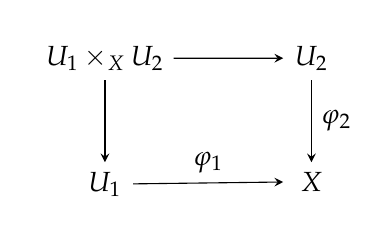
\begin{tikzpicture}
		\matrix (m) [matrix of math nodes,row sep=3em,column sep=4em,minimum width=2em]
		{
			U_1\times_X U_2 & U_2\\ 
			U_1 & X\\};
		\path[-stealth]
		(m-1-1) edge node [above] {} (m-1-2)
		(m-2-1) edge node [above]  {$\varphi_1$} (m-2-2)
		(m-1-1) edge node [right]  {} (m-2-1)
		(m-1-2) edge node [right] {$\varphi_2$} (m-2-2);
	\end{tikzpicture}
	\\
	having the obvious universal property. 
	
\end{definition}
\begin{definition}\label{site_defn}\cite{milne:lec}
	A category $\mathscr C$  
	together with, for each object $U$ of $\mathscr C$, a distinguished set of families of maps $\left\{U_\iota \to U\right\}_{\iota\in I}$, called the \textit{coverings} of $U$, 
	satisfying the following axioms: 
	\begin{enumerate}
		\item[(a)] for any covering $\left\{U_\iota \to U\right\}_{\iota\in I}$ and any morphism $U \to V$ in $\mathscr C$, the fibre products 
		$U_\iota\times_U V$ exist, and $\left\{U_\iota\times_U V \to V\right\}_{\iota\in I}$ is a covering of $V$; 
		\item[(b)] if $\left\{U_\iota \to U \right\}_{\iota\in I}$ is a covering of $U$, and if for each $\iota \in I$, $\left\{V_{\iota j} \to U_\iota  \right\}_{j \in I_\iota}$	is a 
		covering of $U_\iota$, then the family $\left\{V_{\iota j }\to U\right\}_{\iota j}$ is a covering of $U$; 
		\item[(c)] for any $U$ in $\mathscr C$, the family $\left\{U\xrightarrow{\Id}U \right\}$ consisting of a single map is a covering of $U$. 
	\end{enumerate}
	The system of coverings is then called a \textit{Grothendieck topology}, and $\mathscr C$  together with 
	the topology is called a \textit{site}. If $\mathbf T$  
	is a site, then $\mathrm{Cat}\left( \mathbf T\right)$  denotes the underlying category. 
	
\end{definition}
\begin{example}\label{top_gro_exm}
	If $\sX$ is a topological space then one has a category of open subsets and inclusions. If $\sU_1, \sU_2 \subset \sX$ are open set then one can define a fibre product (cf. Definition \ref{pullback_defn}) by the following way
	$$
\sU_1\times_\sX \sU_2 \bydef \sU_1 \cap \sU_2.	
	$$
	If $\sU \subset \sX$ is an open subset then we assume that a family  $\left\{\sU_\iota \to \sU\right\}_{\iota\in I}$, is a covering of $\sU$ (cf. Definition \ref{site_defn}) if and only if  $\sU = \cup_{\iota\in I}\sU_\iota$. This system of coverings is Grothendieck topology.
\end{example}

\begin{definition}\label{etale_presheaf_defn}\cite{milne:lec}
	A \textit{presheaf of sets} on a site $\mathbf T$ 
	is a contravariant functor $\mathscr F$ from $\mathrm{Cat}\left( \mathbf T\right)$ to the category of sets. Thus,  $\mathscr F\left(U \right) $
	to each object $F$ in $\mathrm{Cat}\left( \mathbf T\right)$ 
	attaches a set $\mathscr F\left(U \right)$ , and to each morphism $\phi: U \to V$
	in $\mathrm{Cat}\left( \mathbf T\right)$, a map $\mathscr F\left(\varphi\right):\mathscr F\left(V \right)\to \mathscr F\left(U \right)$. Note that the notion of a presheaf on T 
	does not depend on the 
	coverings. We sometimes denote $\mathscr F\left(\varphi\right)$ by $a \mapsto a|_U$.
	
\end{definition}
Similarly, a presheaf of (Abelian) groups or rings on $\mathbf T$ is a contravariant functor from
$\mathrm{Cat}\left( \mathbf T\right)$ to the category of (Abelian) groups or rings.
\begin{definition}\label{etale_sheaf_defn}\cite{milne:lec}
	A \textit{sheaf} on $\mathbf T$ 
	is a presheaf $\mathscr F$ 
	that satisfies the sheaf condition, that is a sequence 
	\be\label{etale_sheaf_eqn}
	\mathscr F \left(U\right) \to \prod_{\iota \in I} \mathscr F \left(U_\iota \right)\rightrightarrows  \prod_{\iota, j \in I\times I} \mathscr F \left(U_\iota \times_U U_j\right)
	\ee
	is exact for every covering $\left\{U_\iota \to U\right\}$. Thus $\mathscr F$ 
	is a sheaf if the map 
	$$
	f \mapsto \left\{f_{U_\iota }\right\}:\mathscr F \left(U\right) \to \prod_{\iota \in I} \mathscr F \left(U_\iota \right)
	$$
	identifies $\mathscr F\left( U\right)$ with the subset of the product consisting of families $\left\{f_\iota\right\}$such that 
	$$
	f_\iota|_{U_\iota \times_U U_j}= f_j|_{U_\iota \times_U U_j}
	$$
	for all $\iota, j \in I$. 
	When $\mathbf T$ 
	is the site arising from a topological space, these definitions coincide with the 
	usual definitions. 
	
\end{definition}

There are categories $\mathbf{PreSh}\left(\mathbf T \right)$, $ \mathbf{Sh}\left(\mathbf T\right)$ of presheaves an sheaves. Moreover there is a forgetful functor  functor $\mathfrak{Forget} : \mathbf{Sh}\left(\mathbf T \right)\to \mathbf{PreSh}\left(\mathbf T \right)$.

\begin{statement}\label{site_sheaf_stmt}\cite{johnstone:topos}
	There is an adjoint $\mathfrak{Ass} : \mathbf{PreSh}\left(\mathbf T  \right)\to \mathbf{Sh}\left(\mathbf T \right)$ to the given by the forgetful functor $\mathfrak{Forget} : \mathbf{Sh}\left(\mathbf T  \right)\to \mathbf{PreSh}\left(\mathbf T \right)$.
\end{statement}	
\begin{defn}\label{site_sheaf_ass_defn}\cite{johnstone:topos}
	The given by the Statement  \ref{site_sheaf_stmt} functor $\mathfrak{Ass} : \mathbf{PreSh}\left(\mathbf T  \right)\to \mathbf{Sh}\left(\mathbf T \right)$  is said to be an  \textit{associated sheaf functor}.
\end{defn}
\begin{statement}\label{site_enough_stmt}\cite{johnstone:topos}
	%8.13$
	If $\mathbf T$ is site then a category $\mathbf {Ab}\left(\mathbf T \right)$ of sheaves of Abelian groups has enough injectives.
\end{statement}
\begin{definition}\label{grothendiek_topos_defn}\cite{johnstone:topos}
	A category $\mathscr E$ is said to be a \textit{Grothendieck topos} if there exist a site $\mathbf T$ such that $\mathscr E$ is equivalent to a category  $\mathbf{Sh}\left(\mathbf T  \right)$ of sheaves of sets on $\mathbf T$.
\end{definition}


\begin{definition}\label{geom_mor_defn}\cite{johnstone:topos}
	Let $\mathscr E$, $\mathscr F$ be toposes a \textit{geometric morphism} $\mathscr F\xrightarrow{f}\mathscr E$ consists of a pair of functors $\mathscr E\xrightarrow{f_*}\mathscr F$  and $\mathscr E\xrightarrow{f^*}\mathscr F$ such that $f^*$ is left adjoint to $f_*$ and $f^*$ is left exact. 
\end{definition}
\begin{definition}\label{constant_presheaf_defn}\cite{johnstone:topos}
	For any set $A$ there is a \textit{constant presheaf} $\mathscr P$ such that $\mathscr P\left( U\right) = A$ and $\rho^\sU_\sV = \Id_A$ for all $V\subset U$. If $X$ is the terminal object of $\mathrm{Cat}\left( \mathbf T\right)$ (cf. Definition \ref{site_defn})
	then we use a following notation
	\be\label{constant_presheaf_eqn}
	A_X \bydef \mathscr P.
	\ee
\end{definition}

\subsection{Cohomology of sheaves}\label{sheaf_cohomology_sec}\label{grothendieck_cohomology_section}
\paragraph{}
Here I follow to \cite{milne:lec}. The functor
\bean
\Ga\left(X, \cdot \right) : \mathbf {Ab} \left(\mathbf T \right) \to \mathbf {Ab} ,\\
\mathscr F \mapsto \mathscr F\left(X \right) 
\eean
of global sections is left exact, and we define $H^r\left(X,~ \cdot ~\right)$ to be its $r^{\text{th}}$ right derived functor. Explicitly, for a sheaf $\mathscr F$, choose an injective resolution
$$
0 \to \mathscr F \to \mathscr I^0\to \mathscr I^1\to \mathscr I^2 \to ...
$$
and apply the functor $\Ga\left(X, \cdot \right)$ to obtain a complex
\be\label{complex_eqn}
0 \xrightarrow{\dl_0}\Ga\left(X,\ \mathscr I^0  \right) \xrightarrow{\dl_1} \Ga\left(X, \mathscr I^1  \right) \xrightarrow{\dl_2} \Ga\left(X, \mathscr I^2  \right) \to ... 
\ee
This is no longer exact (in general).
 
\begin{theorem}\label{derived_finctor_thm}\cite{hartshorne:ag}
	%			Theorem 1.1 A. 
	Let $\mathfrak A$ be an Abelian category with enough injectives, and let 
	$F: \mathfrak A \to  \mathfrak B$ be a covariant left exact functor to another Abelian category $\mathfrak B$. 
	Then 
	\begin{enumerate}
		\item [(a)] For each $n \ge 0$, $R^nF$ as defined above is an additive functor from  $\mathfrak A$ 
		to $\mathfrak B$. Furthermore, it is independent (up to natural isomorphism of functors) 
		of the choices of injective resolutions made.
		\item[(b)] There is a natural isomorphism $F \cong R^0F$.
		\item[(c)] For each short exact sequence $0 \to A'\to A \to A'' \to 0$ and for each 
		$n \ge 0$ there is a natural morphism $\delta^n R^nF\left(A''\right)\to R^{n +1}F\left(A''\right)$, such that we 
		obtain a long exact sequence 
		$$
		\dots \to R^nF\left(   A'\right) \to R^nF\left(   A\right) \to R^nF\left(   A''\right) \xrightarrow{\delta^n} R^{n+1}F\left(   A'\right) \to  R^{n+1}F\left(   A\right) \to \dots.
		$$
		\item[(d)] Given a morphism of the exact sequence of (c) to another $0\to B'\to B \to B''\to 0$, the $\delta$'s give commutative diagram 
		\newline
		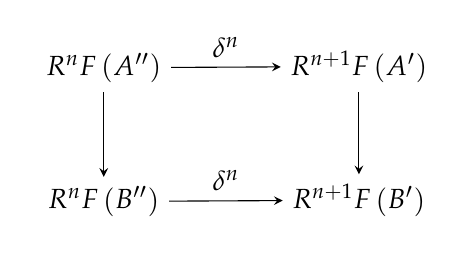
\begin{tikzpicture}
			\matrix (m) [matrix of math nodes,row sep=3em,column sep=4em,minimum width=2em]
			{
				R^nF\left(A''\right) & R^{n+1}F\left(A'\right)\\ 
				R^nF\left(B''\right) & R^{n+1}F\left(B'\right)\\};
			\path[-stealth]
			(m-1-1) edge node [above] {$\delta^n$} (m-1-2)
			(m-2-1) edge node [above]  {$\delta^n$} (m-2-2)
			(m-1-1) edge node [right]  {} (m-2-1)
			(m-1-2) edge node [right] {} (m-2-2);
		\end{tikzpicture}
		\\
		\	
		\item[(e)] For each injective object $I$ of $\mathfrak A$, and for each $n \ge 0$, we have $R^nF\left(I\right)= 0$.
		
	\end{enumerate}
\end{theorem}
The complex \eqref{complex_eqn}  and the Theorem \ref{derived_finctor_thm} define the $r^{\text{th}}$ cohomology
group  
\be\label{etale_coh_eqn}
H^r\left(X,\ \mathscr F \right)\bydef R^r\Ga\left(X, \mathscr F \right)= \ker~ \dl_{r+1} / \im~ \dl_r
\ee
(cf. equation \ref{complex_eqn})
The theory of derived functors (cf. Theorem \ref{derived_finctor_thm}) shows:
\begin{enumerate}
	\item [(a)] $H^0\left(X,\ \mathscr F  \right)\cong \Ga\left(X,\ \mathscr F \right)$ for any sheaf $\mathscr F$;
	\item [(b)] if $\mathscr I$ is injective, then $H^r (X,\mathscr I )= 0$ for $r > 0$;
	\item [(c)]  short exact sequence of sheaves
	$0\to \mathscr F' \to \mathscr F \to \mathscr F'' \to 0$	gives rise to a long exact sequence
	$$
	0 \to H^0\left(X, \mathscr F'  \right) \to H^0\left(X, \mathscr F  \right) \to H^0\left(X, \mathscr F''  \right) \to H^1\left(X,\ \mathscr F'  \right) \to ...
	$$
	and the association of the long exact sequence with the short exact sequence is functional.
\end{enumerate}
Moreover, the functors $H^r\left( X,~ \cdot ~\right)$  are uniquely determined (up to a unique isomorphism)
by the properties (a), (b) and (c).


\begin{proposition}\label{spectral_sequence_prop}\cite{johnstone:topos}
	Let $\mathscr F \xrightarrow{f} \mathscr E$ be a geometric morphism (cf. Definition \ref{geom_mor_defn}) between Grothendieck toposes (cf. Definition \ref{grothendiek_topos_defn}). Then
	\begin{enumerate}
		\item [(i)] If $A$ is an Abelian group in $\mathscr E$ then we have a homomorphism $H^q\left(\mathscr E, A \right) \xrightarrow{} H^q \left(\mathscr F, f^*A\right)$ for each $q$ which is functorial in $f$ and natural in $A$.
		\item [(ii)] If $B$ is an Abelian group in $\mathscr F$ then we have a spectral sequence (Leray spectral sequence) $H^q\left(\mathscr E, R^qf_*\left(B \right) \right)\Rightarrow H^{p + q}\left( B , \mathscr F \right)$ which is natural in $B$.
	\end{enumerate}
\end{proposition}
\begin{notation}\label{const_shef_coh_not}
	If  $F$ is an Abelian group and $F_X$ is a {constant presheaf} (cf. Definition \ref{constant_presheaf_defn}) then we use the following notation
	\be\label{const_shef_coh_eqn}
	\forall r\ge 0\quad H^r\left(X, F \right) \bydef H^r\left(X, \mathfrak{Ass} \left( F_X\right)  \right) 
	\ee
	where $\mathfrak{Ass}$ means the associated sheaf functor (cf. Definition \ref{site_sheaf_ass_defn}).
\end{notation}

\subsection{\v{C}ech cohomology}\label{presheaf_cohomology_sec}
\paragraph{} Here I follow to \cite{milne:lec}. Let $\mathscr U \bydef \left\{U_\iota \to X\right\}_{\iota \in I}$ be  covering of $X$, and let $\mathscr P$ be a presheaf of Abelian groups. Define
\be\label{cech_eqn}
C^r\left( \mathscr U, \mathscr P\right)\bydef \prod_{\left(\iota_0,.... \iota_r\right) \in I^{r+1}} \mathscr P\left(U_{\iota_0,.... \iota_r} \right)\quad \text{where} \quad U_{\iota_0,.... \iota_r} \bydef U_{\iota_0}\times_X...\times_XU_{\iota_r}. 
\ee
For $s \in C^r\left( \mathscr U, \mathscr P\right)$ define $d^rs \in C^{r+1}\left( \mathscr U, \mathscr P\right)$ by the rule
$$
d^rs_{\iota_0,..., \iota_{r + 1}}\bydef \sum_{j = 0}^{r + 1}\left(-1 \right) \mathrm{res}_j\left(s_{\iota_0,..., \iota_{j-1},...,\iota_{j+1},..., \iota_{r + 1}} \right)  
$$
$\mathrm{res}_j$ is the restriction map corresponding to the projection map
$$
U_{\iota_0,..., \iota_{r + 1}}\mapsto U_{\iota_0,..., \iota_{j-1},...,\iota_{j+1},.., \iota_{r + 1}}
$$
In the above construction one has
\be\label{cech_s_eqn}
s_{\iota_0,..., \iota_p}\in U_{\iota_0}\times_X...\times_XU_{\iota_r}
\ee
As in the classical case, one verifies by a straightforward calculation that
$$
C^\bullet\left( \mathscr U, \mathscr P\right) \bydef C^0\left( \mathscr U, \mathscr P\right) \to C^r\left( \mathscr U, \mathscr P\right) \xrightarrow{d_r} C^r\left( \mathscr U, \mathscr P\right)\to ...
$$
is a complex. Define
\be\label{cech_coh_eqn}
\check{H}^r\left( \mathscr U, \mathscr P\right) \bydef H^r\left(C^\bullet\left( \mathscr U, \mathscr P\right)   \right). 
\ee
It is called the $r^{\text{th}}$ \textit{\v{C}ech cohomology group} of $\mathscr P$ relative to the covering $\mathscr U$.
Note that
$$
\check{H}^r\left( \mathscr U, \mathscr P\right)= \ker\left(\prod \mathscr P_\iota \rightrightarrows \prod \mathscr P_{\iota,j} \right) 
$$
Therefore, for a sheaf $\mathscr F$ one has
$$
\check{H}^0\left( \mathscr U, \mathscr F\right)=\Ga\left( \mathscr U, \mathscr F\right).
$$
A second covering $\mathscr V \bydef \left\{V_j\to X \right\}_{j \in J}$ of $X$ is called a \textit{refinement} of $\mathscr U$ if there is a
map $\tau : J\to I$ such that $V_j \to X$ factors through $U_{\tau_j}\to X$ for all $j \in J$ . The choice of
a $\tau$ and $X$-morphisms $\varphi_{j}: V_j \to U_{\tau_j}$ for each $j$ determines a map of complexes
\bean
\tau^\bullet: C^\bullet\left( \mathscr U, \mathscr P\right)\to C^\bullet\left( \mathscr V, \mathscr P\right),\\
\left( \tau^r s_{j_0,..., j_{r}} \right) \bydef s_{\tau j_0,..., \tau j_{r}}.
\eean
As in the classical case, one verifies that the map on cohomology groups
$$
\rho \left(\mathscr U, \mathscr V \right): \check{H}^r\left( \mathscr U, \mathscr P\right)\to \check{H}^r \left( \mathscr V, \mathscr P\right)
$$
is independent of all choices. We may pass to the limit over all coverings, and so obtain limits
\be\label{chech_eqn}
\check{H}^r\left(X, \mathscr P\right)\bydef \varinjlim_{\mathscr U}\check{H}^r\left( \mathscr U, \mathscr P\right).
\ee

\begin{defn}\label{chech_defn}\cite{bryl:loop,milne:lec}
	The  \textit{\v{C}ech cohomology groups} are given by equation \eqref{chech_eqn}
\end{defn}
These groups  have the following properties:
\begin{enumerate}
	\item [(a)] $\check{H}^0\left(X, \mathscr F\right)= \Ga\left( X, \mathscr F\right)$ for any sheaf $\mathscr F$ on $X$;
	\item[(b)] $\check{H}^0\left(X, \mathscr I\right)$, $r > 0$, for all injective sheaves $\mathscr I$.
\end{enumerate}
\begin{empt}
	For any Abelian group $A$ one can define a constant presheaf $A_\sX$ of Abelian groups (cf. Definition \ref{constant_presheaf_defn}). 
	We use a following notation
	\be\label{etale_hom_a_eqn}
	\check{H}^r\left(X,  A\right)\bydef \check{H}^r\left(X, A_\sX\right).
	\ee
\end{empt}


\section{Presheaves and sheaves}
\subsection{General theory}

\begin{definition}\label{presheaf_defn}\cite{hartshorne:ag}
	Let $\sX$ be a topological space. A \textit{presheaf} $\mathscr F$ of Abelian groups on  $\sX$ consists of the data
	\begin{itemize}
		\item[(a)] for every open subset $\sU \subseteq \sX$, an Abelian group $\mathscr F\left(\sU\right)$, and 
		\item[(b)] for every inclusion $\sV \subseteq \sU$ of open subsets of $\sX$, a morphism of Abelian groups $\rho_{\sU \sV}:\mathscr F\left(\sU\right) \to \mathscr F\left(\sV\right)$,\\
		subject to conditions
		\begin{itemize}
			\item [(0)] $\mathscr F\left(\emptyset \right)= 0$, where $\emptyset$ is the empty set,
			\item[(1)] $\rho_{\sU \sU}$ is the identity map, and
			\item[(2)] if $\mathcal W \subseteq \sV \subseteq \sU$ are three open sets, then $\rho_{\sU \mathcal W} = \rho_{\sV \mathcal W }\circ \rho_{\sU \sV}$.
		\end{itemize}
	\end{itemize}
\end{definition}

\begin{definition}\label{sheaf_defn}\cite{hartshorne:ag}
	A \textit{presheaf} $\mathscr F$ on  
	a topological space $\sX$ is a \textit{sheaf}  if it satisfies the following supplementary conditions:
	\begin{itemize}
		\item[(3)] If $\sU$ is an open set, if $\left\{\sV_{\a}\right\}$ is an open covering of $\sU$, and if $s \in \mathscr F\left(\sU\right)$ is an element such that $\left.s\right|_{\sV_{\a}}= 0$ for all $\a$, then $s = 0$;
		\item[(4)] If $\sU$ is an open set, if $\left\{\sV_{\a}\right\}$ is an open covering of $\sU$ (i.e. $\sU = \cup\sV_\a$), and we have elements $s_\a$ for each $\a$, with property that for each $\al, \bt, \left.s_\a\right|_{\sV_{\a}\cap \sV_{\bt}}= \left.s_\bt\right|_{\sV_{\a}\cap \sV_{\bt}}$, then there is an element $s \in \mathscr F\left(\sU\right)$ such that $\left.s\right|_{\sV_\a} = s_\a$ for each $\a$.
	\end{itemize}
	(Note condition (3) implies that $s$ is unique.)
\end{definition}


\begin{remark}
From the Example \ref{top_gro_exm} it follows that the Definitions \ref{presheaf_defn} and  \ref{sheaf_defn} a specializations of  \ref{etale_presheaf_defn} and  \ref{etale_sheaf_defn} ones.
\end{remark}
%\begin{definition}
%	A presheaf \ref{top_x_sheaf_defn} satisfying (4) of the Definition \ref{sheaf_defn} is called \textit{conjunctive} (for $\sU$). (cf. \cite{bredon:sheaf})
%\end{definition}
\begin{definition}\label{stalk_defn}\cite{hartshorne:ag}
	If $\mathscr F$ is a {presheaf} on $\sX$, and if $x$ is a point of $\sX$ we define the \textit{stalk} or the \textit{germ} $\mathscr F_x$ of $\mathscr F$ at $x$ to be the direct limit of groups $\mathscr F\left(\sU\right)$ for all open sets $\sU$ containing $x$, via restriction maps $\rho$.
\end{definition}

\begin{definition}\cite{hartshorne:ag}
	If $\mathscr F$  and $\mathscr G$ are presheaves on $\sX$, a \textit{morphism} $\varphi:\mathscr F\to\mathscr G$  consists 
	of a morphism of Abelian groups $\varphi_\sU:\mathscr F\left( \sU\right) \to\mathscr F\left( \sU\right)$ for each open set 
	$\sU$, such that whenever $\sV\subset\sU$ is an inclusion, the diagram 
	\newline
	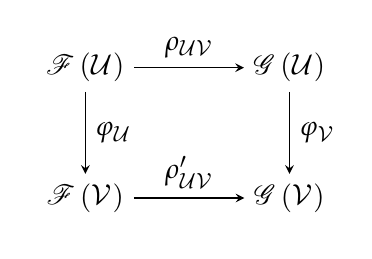
\begin{tikzpicture}
		\matrix (m) [matrix of math nodes,row sep=3em,column sep=4em,minimum width=2em]
		{
			\mathscr F\left( \sU\right)   & \mathscr G\left( \sU\right)\\
			\mathscr F\left( \sV\right)    & \mathscr G\left( \sV\right)\\
		};
		\path[-stealth]
		(m-1-1) edge node [above] {$\rho_{\sU\sV}$} (m-1-2)
		(m-1-1) edge node [right] {$\varphi_\sU$} (m-2-1)
		(m-1-2) edge node [right] {$\varphi_\sV$} (m-2-2)
		(m-2-1) edge node [above] {$\rho'_{\sU\sV}$} (m-2-2);
	\end{tikzpicture}
	\\
	is commutative, where $\rho_{\sU\sV}$ and $\rho'_{\sU\sV}$ are the restriction maps in $\mathscr F$  and $\mathscr G$. If $\mathscr F$  and $\mathscr G$ are sheaves on $\sX$, we use the same definition for a morphism 
	of sheaves. An isomorphism is a morphism  which has a two-sided inverse. 
\end{definition}

\begin{prdf}\label{sheaf_prdf}\cite{hartshorne:ag}
	Given a presheaf $\mathscr F$, there is a sheaf  $\mathscr F^+$ and a morphism $\th: \mathscr F \to \mathscr F^+$, with the property that for any sheaf  $\mathscr G$, and any morphism $\varphi: \mathscr F \to \mathscr G$, there is a unique morphism $\psi:\mathscr F^+\to \mathscr G$ such that $\varphi = \psi \circ \th$. Furthermore the pair $\left(\mathscr F^+, \th\right)$ is unique up to unique isomorphism. $\mathscr F^+$ is called the $\mathrm{sheaf~associated}$ to the presheaf $\mathscr F$. 
\end{prdf}

\begin{exercise}\label{sheaf_etale_exer}\cite{hartshorne:ag}
	%1.13. 
	\textit{
		\'Espace Etal\'e of a Presheaf}. %(This exercise is included only to establish the connection between our definition of a sheaf and another definition often found in the literature. See for example Godement [1, Ch. II, �1.2].)
	Given a presheaf $\mathscr F$ on $\sX$, we define a topological space $\mathrm{Sp\acute{e}}\left(\mathscr F \right)$ , called the \textit{
		\'espace etal\'e} of a presheaf of $\mathscr F$ as 
	follows. As a set, $\mathrm{Sp\acute{e}}\left(\mathscr F \right)= \bigcup_{x\in\sX} \mathscr F_x$. We define a projection map $p: \mathscr \mathrm{Sp\acute{e}}\left(\mathscr F \right)$
	by sending $s_x\in \mathscr F_x$ to $x$. For each open set $\sU\subset\sX$ and each section $s\in \mathscr F\left(\sU \right)$  we 
	obtain a map: $\overline{s}: \sU \to  \mathrm{Sp\acute{e}}\left(\mathscr F \right)$ by sending $x \mapsto s_x$, its germ at $x$. This map has the property that 
	$p\circ \overline{s}= \Id_\sX$, in other words, it is a "section" of $p$ over $\sU$. We now 
	make $\mathrm{Sp\acute{e}}\left(\mathscr F \right)$ into a topological space by giving it the strongest topology such that 
	all the maps $\overline{s}: \sU \to  \mathrm{Sp\acute{e}}\left(\mathscr F \right)$ for all $\sU$ and all $s\in \mathscr F\left(\sU \right)$ , are continuous. Now 	show that the sheaf $\mathscr F^+$ associated to $\mathscr F$ can be described as follows: for any 
	open set $\sU\subset \mathscr F$, $\mathscr F\left(\sU \right)$ is the set of continuous sections of $\mathrm{Sp\acute{e}}\left(\mathscr F \right)$ over $\sU$. In 
	particular, the original presheaf $\mathscr F$ was a sheaf if and only if for each $\sU\subset \sX$,  $\mathscr F\left(\sU \right)$ is 
	equal to the set of all continuous sections of $\mathrm{Sp\acute{e}}\left(\mathscr F \right)$ over $\sU$. 
	
\begin{exercise}\label{sheaf_etale_open_exer}
\end{exercise}
Let $s \in \mathscr F\left(\sU\right)$ be a section. Prove following statements.
\begin{enumerate}
	\item The set 
	\be\label{sheaf_u_s_eqn}
\mathscr U_s\bydef \left\{s_x\right\}_{x \in \sU}
	\ee
is open subset  of the \'espace etal\'e  of $\mathrm{Sp\acute{e}}\left(\mathscr F \right)$ of the presheaf $\mathscr F$.
	\item The family  of all given by the equation \eqref{sheaf_u_s_eqn} sets $\mathscr U_s$ is basis of the topology of  $\mathrm{Sp\acute{e}}\left(\mathscr F \right)$.
	\item The natural continuous map $\mathrm{Sp\acute{e}}\left(\mathscr F \right)\to\sX$ is open.
	\end{enumerate}
\end{exercise}

\begin{definition}\label{sheaf_inv_im_defn}\cite{hartshorne:ag}
	Let $f: \sX\to \sY$ be a continuous map of topological spaces. For any sheaf  $\mathscr F$ on $\sX$, we define the \textit{direct image} sheaf  $f_*\mathscr F$ on $\sY$ by $\left(f_*\mathscr F\right)\left(\sV\right)= \mathscr F\left(f^{-1}\left(\sV\right)\right)$ for any open set $\sV \subseteq \sY$. For any sheaf  $\mathscr G$ on $\sY$, we define the \textit{inverse image} sheaf  $f^{*}\mathscr G$ on $\sX$ be the sheaf  associated to the presheaf  $\sU \mapsto \lim_{\sV \supseteq f\left(\sU\right)} \mathscr G\left(\sV\right)$, where $\sU$ is any open set in $\sX$, and the limit is taken over all open sets $\sV$ of $\sV$ containing $f\left(\sU\right)$.
\end{definition}

\begin{remark}\label{geometric_morphism_rem}\cite{johnstone:topos}
	%1.17
	If $f : \sX \to \sY$ is a continuous map then a given by the Definition \ref{sheaf_inv_im_defn} pair  of functors $f_*$ and $f^{*}$ rise a geometric morphism (cf. Definition \ref{geom_mor_defn}) $\mathbf{Sh}\left(\sY\right)\to \mathbf{Sh}\left(\sX\right)$ between categories of sheaves. 
\end{remark}
\subsection{Cohomology}
\paragraph{}
From the Example \ref{top_gro_exm} it follows that both Definitions \ref{presheaf_defn} and \ref{sheaf_defn} are specializations of  \ref{etale_presheaf_defn} and \ref{etale_sheaf_defn} ones. So for any topological space $\sX$ there are theories of cohomology explained in sections \ref{sheaf_cohomology_sec} and \ref{presheaf_cohomology_sec}
\begin{lemma}\cite{hartshorne:ag}
	Let $\sX$ be a topological space, and $\mathscr U$ an open covering of $\sX$. Then for any sheaf $\mathscr U$ on $\sX$ and
	for each $r \ge 0$ there is a natural map, functorial in $\mathscr F$.
	$$
	\check{H}^r\left(\mathscr U, \mathscr F \right) \to H^r\left( \sX, \mathscr F\right) 
	$$
	where both $\check{H}^r$ and $H^r$ are given by the equations \eqref{cech_coh_eqn} and \eqref{etale_coh_eqn} respectively.
\end{lemma}
\begin{remark}
From the above lemma and the equation  \ref{chech_eqn} for each $r\ge 0$ one has a homomorphism
$$
\check{H}^r\left(\sX, \mathscr F \right) \to H^r\left( \sX, \mathscr F\right).
$$
\end{remark}
\begin{remark}
If $f: \sX \to \sY$ is a continuous map and $A$ is an Abelian group then from the Remark \ref{geometric_morphism_rem} and  the Proposition \ref{spectral_sequence_prop} for any $r> 0$ there is a natural homomorphism
\be\label{hom_f_eqn}
H^r\left(f \right) : H^r\left(\sY, A \right) \to H^r\left(\sX, A \right)
\ee
where the notation \eqref{const_shef_coh_not} is used.
\end{remark}
\begin{empt}
If $f: \sX\to\sY$ is a continuous map  $\mathscr U = \left\{\sU_\iota\right\}_{\iota} \in I$ is a covering of $\sX$ (cf. Definition \ref{site_defn} and Example \ref{top_gro_exm}) then a family $f^{-1}\left(\mathscr U \right) \bydef \left\{f^{-1}\left( \sU_\iota\right) \right\}_{\iota} \in I$ is a covering of $\sY$. Let $A$ be a Abelian group, and let $\mathscr P_\sX$, $\mathscr P_\sY$ be a corresponding constant presheaves (cf. Definition \ref{constant_presheaf_defn}) on $\sX$ and $\sY$.  Following equation
\be\label{top_cech_eqn}
C^r\left( \mathscr U, \mathscr P_\sX\right)\bydef \prod_{\left(\iota_0,.... \iota_r\right) \in I^{r+1}} \mathscr P_\sX\left(\sU_{\iota_0,.... \iota_r} \right)\quad \text{where} \quad \sU_{\iota_0,.... \iota_r} \bydef \sU_{\iota_0}\cap...\cap \sU_{\iota_r}. 
\ee
is a specialization of \eqref{cech_eqn} one (cf. Example \ref{top_gro_exm}. For any $\left(\iota_0,.... \iota_r\right) \in I^{r+1}$ one has an isomorphism
$$
\mathscr P_\sX\left(\sU_{\iota_0,.... \iota_r} \right)\cong \mathscr P_\sY\left(f^{-1}\left( \sU_{\iota_0,.... \iota_r} \right)\right) \cong A.
$$
Above isomorphisms yield an isomorphism
$$
C^r\left( f^{-1}\left( \mathscr U\right) , \mathscr P_\sY\right)\cong C^r\left( \mathscr U, \mathscr P_\sX\right).
$$
From these isomorphisms  one can obtain a natural homomorphism
$$
\check{H}^r\left(f\right):\check{H}^r\left(\sY, \mathscr P_\sY \right)\to \check{H}^r\left(\sX, \mathscr P_\sX \right)\quad r \ge 0.
$$
The details of the construction of the homomorphism $\check{H}^r\left(f\right)$  are explained in \cite{eust}. Using the Notation \ref{constant_presheaf_defn} one has
\be\label{cech_hom_eqn}
\begin{split}
\check{H}^r\left(f\right):\check{H}^r\left(\sY, A \right)\to \check{H}^r\left(\sX, A \right)\quad r \ge 0,\\
\check{H}^\bullet\left(f\right):\check{H}^\bullet\left(\sY, A \right)\to \check{H}^\bullet\left(\sX, A \right).
\end{split}
\ee

\end{empt}








\begin{empt}\label{tens_prop_c_empt}\cite{bryl:loop}
\v{C}ech cohomology has the advantage of allowing an easy and explicit construction of a \textit{cup}-\textit{product}
$$
\check{H}^p\left(\mathscr U,  \mathscr F\right) \otimes \check{H}^q\left(\mathscr U,  \mathscr G\right)\to \check{H}^p\left(\mathscr U,  \mathscr F\otimes \mathscr G\right).
$$
		Here $\mathscr F$ and $\mathscr G$ are sheaves of Abelian groups on $\sX$, and the \textit{tensor product}- \textit{sheaf}
	 $\mathscr F\otimes \mathscr G$ is the sheaf associated to the presheaf $\sU \mapsto \mathscr F(\sU)\otimes \mathscr G(\sU)$. The 
		stalk (cf. Definition \ref{stalk_defn}) at $x$ of $\mathscr F\otimes \mathscr G$ is $\mathscr F_x\otimes \mathscr G_x$ The cup-product will be defined from a 
		morphism of complexes. We first need the notion of tensor product $A^\bullet \otimes  B^\bullet$
		of two complexes; this is the total complex of the double complex $A^\bullet \otimes  B^\bullet$. 
		So the degree $n$-term of$A^\bullet \otimes  B^\bullet$ is $\oplus A^p\otimes B^{n-p}$. The differential in $A^\bullet \otimes  B^\bullet$.  
		is 
		$$
	d \left(a \otimes b\right)	\bydef \left(da\right)\otimes b + \left(-1\right)^p a \otimes db
		$$
		
	for $a\in A^p$, $b \in B^q$. We have the obvious 
		tensor product 
	$$
\otimes :H^p\left(A^\bullet\right)\otimes H^q\left(B^\bullet\right)\to H^q\left(B^\bullet\right).	
	$$	
	We now return to the sheaves $\mathscr F$ and $\mathscr G$ of Abelian groups on $\sX$. We 
		have the complexes $C^\bullet\left(\mathscr U,  \mathscr F\right)$ and $C^\bullet\left(\mathscr U,  \mathscr G\right)$  The interesting part is the 
		construction of a morphism of complexes 
	$$
\phi: C^\bullet\left(\mathscr U,  \mathscr F\right)\otimes C^\bullet\left(\mathscr U,  \mathscr G\right)\mapsto C^\bullet\left(\mathscr U,  \mathscr , \mathscr G\right)
	$$
		For $\a \in C^\bullet\left(\mathscr U,  \mathscr F\right)$ and $\bt \in C^\bullet\left(\mathscr U,  \mathscr G\right)$, we put 
	$$
	\phi:\left( \a \otimes \bt \right)_{\iota_0,..., \iota_{p + q}} \bydef \a_{\iota_0,...,\iota_p}\otimes  \bt_{\iota_{p},..., \iota_{p+q}}.
	$$
			One checks easily that $\phi$ is indeed a morphism of complexes. The induced map on cohomology gives the cup-product on \v{C}ech 
			cohomology. For $\a$ degree $p$ \v{C}ech cocycle with coefficients in $\mathscr F$ and $\bt$
			degree $q$ \v{C}ech cocycle with coefficients in $\mathscr G$, we have 
			$$
		\left(\a \smile\bt \right)_{\iota_0,..., \iota_{p + q}}\bydef  \a_{\iota_0,...,\iota_p}\otimes  \bt_{\iota_{p},..., \iota_{p+q}}.
		$$
			The cup-product has the following properties. 
		\end{empt}
		\begin{proposition}\label{cup_ass_prop}\cite{bryl:loop} Following conditions hold.
		%	1.3.7. Proposition. 
		\begin{enumerate}
			\item[(i)] The cup-product is associative, i.e., for $\a \in \check{H}^p\left(\mathscr U,  \mathscr F\right)$,  $\bt \in \check{H}^q\left(\mathscr U,  \mathscr G\right)$, $\ga \in \check{H}^r\left(\mathscr U,  \mathscr H\right)$
	 we have 
	 $$
\a \smile \left( \bt \smile \ga\right) 	= \left( \a \smile \bt\right) \smile \ga. 
	 $$
	 	\item[(ii)]	 The \textit{cup}-\textit{product} is \textit{graded}-\textit{commutative}. If $\a \in \check{H}^p\left(\mathscr U,  \mathscr F\right)$,  $\bt \in \check{H}^q\left(\mathscr U,  \mathscr G\right)$, we have 
$$
\a \smile \bt =\left( -1\right)^p  \bt \smile \a.
$$			
			
		\end{enumerate}
			
	\end{proposition}
	\begin{empt}
		Let $\sX$ be a topological space. If $A$ be an Abelian group then there is, a corresponding constant presheaf  $\mathscr P$ (cf. Definition \ref{constant_presheaf_defn}) on $\sX$. A  presheaf $\mathscr P\otimes \mathscr P$ on $\sX$ is a constant presheaf of a group $A \otimes_Z A$.  A homomorphism $A \otimes_Z A \to  A$ naturally yields a homomorphism $\mathscr P\otimes \mathscr P\to \mathscr P$ of sheaves which induces a homomorphism
		$$
\phi: \check{H}^\bullet\left(\sX, \mathscr P\otimes \mathscr P \right)\to \check{H}^\bullet\left(\sX, \mathscr P \right).
		$$
		Using the cup product and homomorphism $\phi$ one has a map
	$$
	\check{H}^\bullet\left(\sX, \mathscr P \right)\otimes \check{H}^\bullet\left(\sX, \mathscr P \right) \to \check{H}^\bullet\left(\sX, \mathscr P \right).
	$$
	So we have proved the following.	
	\end{empt}
	
	\begin{lem}
		Let $\sX$ be a topological space. If $A$ is an Abelian group then any homomorphism $A \otimes_Z A \to  A$ yields a product
		\bean
		\smile: \check{H}^\bullet\left(\sX, A \right)\otimes \check{H}^\bullet\left(\sX,A \right) \to \check{H}^\bullet\left(\sX,A \right)
		\eean
		where the Notation \eqref{etale_hom_a_eqn} is used. So $\check{H}^\bullet\left(\sX, A \right)$ is an associative and graded-commutative ring.
	\end{lem}
	
	\begin{exercise}
	Let  $A$ be an Abelian group with a homomorphism $A \otimes_Z A \to  A$. Prove that a given by \eqref{cech_hom_eqn} map $\check{H}^\bullet\left(f\right):\check{H}^\bullet\left(\sY, A \right)\to \check{H}^\bullet\left(\sX, A \right)$ is a homomorphism of rings.
	\end{exercise}
	\begin{theorem}\label{homol_tens_prod}\cite{dimca:sheaves}
		%Theorem 2.2.6 
		(K\"{u}nneth Formula). Let $A$ be a principal ideal domain 
		and let $X^\bullet, Y^\bullet$ be two complexes 
		such that $X^\bullet$ is torsion free. Then there are natural exact sequences for any 
		integer $m \in \Z$ 
		\bean
		0\hookto\bigoplus_{p + q = m} H^q\left( X^\bullet\right)\otimes_A H^p\left( Y^\bullet\right)\hookto  H^m\left(X^\bullet \otimes_A Y^\bullet  \right) \to\\\to \bigoplus_{p + q = m-1} Tor_A\left( H^q\left( X^\bullet\right)\otimes H^p\left( Y^\bullet\right)\right) \to 0
		\eean
		
	\end{theorem}
	\begin{empt}
If both $\sX$ and $\sY$ are topological; spaces and both $\mathscr{U}$, and $\mathscr{V}$ are coverings of $\sX$ and $\sY$ (cf. Definition \ref{site_defn}) then there is a natural covering $\mathscr{U}\times\mathscr{V}$ of $\sX \times \sY$.  If $\Z_\sX$ and $\Z_\sY$ are constant presheaves given by the equation \eqref{constant_presheaf_eqn} then one has
$$
C^\bullet \left(\mathscr{U}\times\mathscr{V}, \Z_{\sX\times\sY} \right) = C^\bullet \left(\mathscr{U}, \Z_{\sX} \right)\otimes_\Z C^\bullet \left(\mathscr{V}, \Z_{\sY} \right)
$$
where complexes are given by \eqref{cech_eqn} and a tensor product of complexes is explained in \ref{tens_prop_c_empt}. From the Theorem \ref{homol_tens_prod} one has an injective homomorphism
$$
\bigoplus_{p + q = m}\check{H}^q\left(\mathscr{U}, \Z_{\sX} \right)\otimes \check{H}^p\left( \mathscr{V}, \Z_{\sY} \right)\hookto  \check{H}^m\left((\mathscr{U}\times\mathscr{V}, \Z_{\sX\times\sY} \right).
$$
Using the equation \ref{chech_eqn} one has a following injective homomorphism
\be\label{kunnet_eqn}
\bigoplus_{p + q = m}\check{H}^q\left(\sX, \Z \right)\otimes \check{H}^p\left(\sY, \Z \right)\hookto  \check{H}^m\left(\sX\times\sY, \Z \right)
\ee
where the notation \eqref{etale_hom_a_eqn} is used.
	\end{empt}
		
\section{$C^*$-algebras}
\paragraph*{}  A notion of $C^*$-algebra is explained in \cite{murphy, pedersen:ca_aut, rae:ctr_morita}.
\begin{definition}\label{top_net_defn}\cite{engelking:general_topology}
	A \textit{net in topological space} $\mathcal{ X}$ is an arbitrary function from a non-empty directed set $\La$  to the space $\mathcal{ X}$. Nets will be denoted by $S = \left\{x_\la \in \mathcal{ X}\right\}_{\la \in \La}$. 
\end{definition}




\subsection{Representations of $C^*$-algebras}
\begin{definition}\label{faithful_repr_defn}\cite{murphy}
	A representation $\rho : A\to B\left( \H\right)$ is called \textit{faithful} if the *-homomorphism $\rho$ is injective.
\end{definition}



\begin{theorem}\label{irred_thm}\cite{pedersen:ca_aut}
	Let $\pi: A \to B\left(\H \right)$ be a nonzero representation of $C^*$-algebra $A$. The following conditions are equivalent:
	\begin{enumerate}
		\item [(i)] there are no non-trivial $A$-subspaces for $\pi$,
		\item[(ii)] the commutant of $\pi\left(A \right)$ is the scalar multipliers of 1,
		\item[(iii)] $\pi\left(A \right)$ is strongly dense in   $B\left(\H \right)$,
		\item[(iv)] for any two vectors $\xi, \eta \in \H$ with $\xi \neq 0$ there is $a \in A$ such that $\pi\left(a \right)\xi = \eta$,
		\item[(v)] each nonzero vector in $\H$ is cyclic for  $\pi\left(A \right)$,
		\item[(vi)]  $A \to B\left(\H \right)$ is spatially equivalent to a cyclic representation associated with a pure state of $A$.
	\end{enumerate} 
\end{theorem}
\begin{definition}\label{irred_defn}\cite{pedersen:ca_aut}
	Let $A \to B\left(\H \right)$ be a nonzero representation of $C^*$-algebra $A$. The representation is said to be \textit{irreducible} if it satisfies to the Theorem \ref{irred_thm}.
\end{definition}



\begin{definition}\label{nondegenerate_repr_defn}\cite{matro:hcm}
	A representation $\rho : A\to B\left( \H\right)$ is called \textit{nondegenerate} if for any $\xi \in \H$  there exists an element $a \in A$ such that $\rho\left(a \right)\xi \neq 0$. 
\end{definition}


\begin{definition}\label{atomic_repr_defn}\cite{pedersen:ca_aut}
	Let $A$ be a $C^*$-algebra with the spectrum $\hat A$. We choose for any $t \in \hat A$ a pure state $\phi_t$ and  associated representation $\pi_t: A \to B\left(\H_t\right)$.
	The representation 
	\be
	\pi_a = \bigoplus_{t \in \hat A} \pi_t \quad \text{on the closure } \H_a \text{ of an algebraic direct sum}\quad  \bigoplus_{t \in \hat A} \H_t
	\ee
	is called the (reduced) \textit{atomic representation} of $A$. Any two atomic representations are unitary equivalent and any atomic representation of $A$ is faithful and nondegenerate  (cf.  Definitions \ref{faithful_repr_defn}, \ref{nondegenerate_repr_defn} and \cite{pedersen:ca_aut}).
\end{definition}

\subsection{Hereditary $C^*$-subalgebras}

	\begin{definition}\label{hered_defn}\cite{pedersen:ca_aut}
	A cone $M$ in the positive part of $C^*$-algebra $A$ is said to be \textit{hereditary} if $0 \le x \le y$, $y \in M$ implies $x \in M$ for each $x \in A$. A *-subalgebra $B$ of $A$ is \textit{hereditary} if $B_+$ is hereditary in $A_+$.
\end{definition}
\begin{lemma}\label{hered_lem}\cite{murphy}
	Let $B$ be a $C^*$-subalgebra of $C^*$-algebra $A$. Then $B$ is hereditary in $A$ if and only if $bab' \in B$ for all $b, b' \in B$ and $a \in A$.
\end{lemma}
%\begin{lemma}\label{hered_ideal_lem}\cite{murphy}
%	Let $A$ be a $C^*$-algebra.
%	\begin{enumerate}
%		\item[(i)] If $L$ is a closed left ideal in $A$ then $L\cap L^*$ is a hereditary $C^*$-subalgebra of $A$. The map $L \mapsto L\cap L^*$ is the bijection from the set of closed left ideals of $A$ onto the the set of hereditary $C^*$-subalgebras of $A$.
%		\item[(ii)] If $L_1, L_2$ are closed left ideals, then $L_1 \subseteq L_2$ is and only if $L_1\cap L_1^* \subset L_2\cap L_2^*$.
%		\item[(iii)] If $B$ is a hereditary $C^*$-subalgebra of $A$, then the set 
%		$$
%		L\left(B \right) = \left\{\left.a \in A~\right| a^*a \in B \right\}
%		$$
%		is the unique closed left ideal of $A$ corresponding to $B$.
%	\end{enumerate}
%\end{lemma}


\begin{remark}\cite{murphy}
	Obviously, $0$ and
	$A$ are hereditary $C^*$-subalgebras of $A$, and any intersection of hereditary
	$C^*$-subalgebras is one also. 
	
\end{remark}
\begin{definition}\label{hered_gen_defn}\cite{murphy}
	The hereditary $C^*$-subalgebra \textit{generated} by a
	subset $S$ of $A$ is the smallest hereditary $C^*$-subalgebra of $A$ containing $S$.
\end{definition}
\subsection{Topologies of $C^*$-subalgebras}

	\begin{defn}\label{strict_topology_defn}\cite{pedersen:ca_aut}
	Let $A$ be a $C^*$-algebra.  The {\it strict topology} on the multiplier algebra $M(A)$ is the topology generated by seminorms 
	\be\label{strict_topology_norm_eqn}
	\vertiii{x}_a\bydef \|ax\| + \|xa\|,\quad a\in A.
	\ee
	If $\La$ is a directed set and $\left\{a_\la\in M\left( A\right) \right\}_{\la\in \La}$ is a net the we denote by $\bt\text{-}\lim_{\la\in\La }a_\la$ the limit of $\left\{a_\la \right\}$ with respect to the strict topology.
\end{defn}


\begin{defn}\label{commutant_defn}
	%2.2.1. 
	For each subset $M$ of $B(\H)$ let $M'$ denote the \textit{commutant} of $M$, i.e. 
	\bean
	M'\bydef \left\{b \in B\left(\sH\right)|\forall a \in M \quad ab = ba \right\}
	\eean
	The $C^*$-algebra 
	\bean
	M''\bydef (M')'
	\eean
	is said to be a \textit{bicommutant} of $M$.
\end{defn}
	\begin{lemma}\label{increasing_convergent_w_lem}\cite{pedersen:ca_aut} Let $\Lambda$ be an increasing in the partial ordering.  Let $\left\{x_\lambda \right\}_{\la \in \La}$ be an increasing of self-adjoint operators in $B\left(\H\right)$, i.e. $\la \le \mu$ implies $x_\la \le x_\mu$. If $\left\|x_\la\right\| \le \ga$ for some $\ga \in \mathbb{R}$ and all $\la$ then $\left\{x_\lambda \right\}$ is strongly convergent to a self-adjoint element $x \in B\left(\H\right)$ with $\left\|x_\la\right\| \le \ga$.
\end{lemma}
	\begin{thm}\label{von_Neumann_thm}\cite{pedersen:ca_aut}
	Let $M$ be a $C^*$-subalgebra of $B(\H)$, containing the identity operator. The following conditions are equivalent:
	\begin{itemize}
		\item $M=M''$ where $M''$ is the bicommutant of $M$;
		\item $M$ is weakly closed;
		\item $M$ is strongly closed.
	\end{itemize}
\end{thm}




\begin{lemma}\label{hered_repr_lem}\cite{pedersen:ca_aut}
	%4.1.5. LEMMA. 
	Let $B$ be a hereditary $C^*$-subalgebra of $A$. For each irreducible 
	representation $\pi: A \to B\left( \H\right)$  such that $B \not\subset\ker\pi$ the map $\pi|_B: B \to \pi\left(B \right)\H$  is an irreducible 
	representation of $B$. 
	
\end{lemma}
\begin{proof}
	Let $\left\{u_\la\right\}$ be an approximate unit for $B$ and let $p$ be the projection on the 
	closure of $\pi\left(B \right)\H$ . Then $\left\{\pi\left( u_\la\right) \right\}$ is strongly convergent to $p$. For any pair of vectors $\xi, \eta\in p\H$ with $\xi \neq 0$ there is by  an element $x \in A$ with $\pi\left(x \right)\xi   = \eta$ (cf. Theorem \ref{irred_thm}). But $u_\la x u_\la \in B$ and 
	$$
	\left\|\pi\left(u_\la x u_\la \right) \xi - \eta \right\|\to \left\|p\pi\left( x  \right)p \xi - \eta \right\| = 0.
	$$
	Consequently $\pi\left( B\right)$  acts topologically irreducibly on $p\H$. But then it also acts 
	algebraically irreducibly, so there must be a $y$ in $B$ for which $\pi\left( y\right)\xi  = \eta$. In 
	particular,  $\pi\left( B\right)\H$  is closed and $\pi|_B: B \to \pi\left(B \right)\H$ is irreducible. 
\end{proof}



\subsection{Approximate units}
	\begin{defn}
	\label{strong_topology_defn}\cite{pedersen:ca_aut} Let $\H$ be a Hilbert space. The {\it strong} topology on $B\left(\H\right)$ is the locally convex vector space topology associated with the family of seminorms of the form $x \mapsto \|x\xi\|$, $x \in B(\H)$, $\xi \in \H$.
\end{defn}

\begin{defn}\label{approximate_unit_defn} \cite{pedersen:ca_aut}
	Let $A$ be a $C^*$-algebra. A net $\left\{u_\la \right\}_{\la \in \La}$ in $A_+$ with $\left\|u_\la \right\| \le 1$ for all $\la \in \La$ is called an \textit{approximate unit} for $A$ if $\la < \mu$ implies $u_\la < u_\mu$ and if $\lim \left\|x- xu_\la \right\| = 0$ for each $x$ in $A$. Then, of course, $\lim \left\|x- u_\la x \right\| = 0$ as well.
\end{defn}
\begin{theorem}\label{left_ideal_thm}\cite{murphy}
	%3.1.2. Theorem.
	If $L$ is a closed left ideal in a $C^*$-algebra $A$, then there
	is an increasing net $\left\{u_\la\right\}_{\la\in\La}$ of positive elements in the closed unit ball of
	$L$ such that $a = \lim_{\la\in \La}au_\la $ for all $a\in L$.
\end{theorem}

\begin{thm}\label{approximate_unit_thm} \cite{pedersen:ca_aut}
	Each $C^*$-algebra contains an \textit{approximate unit}.
\end{thm}
\subsection{Continuous trace $C^*$-algebras}	
\begin{definition}\label{continuous_trace_c_alt_defn}\cite{rae:ctr_morita}
	%Definition 5.13. 
	A \textit{continuous-trace} $C^*$-\textit{algebra} is a $C^*$-algebra $A$ with Hausdorff
	spectrum $\sX$ such that, for each $x_0\in\sX$ there are a neighborhood $\sU$ of $x_0$ and $a\in A$ such that $\rho_{ x}\left( a\right) $ is a rank-one projection for all $x \in \sU$, where $\rho_{ x}: A \to B\left(\H_x\right)$ is a corresponding to $x$ irreducible representation.
\end{definition}

\begin{lemma}\label{ctr_rep_eq_lem}\cite{rae:ctr_morita}
	Suppose $A$ is a $C^*$-algebra with Hausdorff spectrum $\mathcal{X}$ and for all $x \in \sX$ $\pi_x : A \to B\left(\H_x \right)$ is a corresponding  to $x$ irreducible representation.
	\begin{itemize}
		\item [(a)] If $a, b \in A$ and $\pi_x\left(a \right)=  \pi_x\left(b \right)$ for every $x \in  \mathcal{X}$, then $a = b$.
		\item[(b)] For each $a \in A$ the function $x \mapsto \left\|\pi_x\left(a \right) \right\|$ is continuous on  $\mathcal{X}$, vanishes at infinity and has sup-norm equal to $\left\| a\right\|$. 
	\end{itemize}
\end{lemma}
\begin{prop}\label{ctr_hered_prop}\cite{pedersen:ca_aut}
	% 6.2.10. PROPOSITION. 
	Each hereditary $C^*$-subalgebra and each quotient of a 
	$C^*$-algebra which  has continuous trace has 
	continuous trace. 
\end{prop}

\begin{proposition}\label{ctr_lt_prop}\cite{cuntz_meyer_ros:bivariant}
	%Proposition 9.3. 
	Let $\H$ be a Hilbert space, and let $\K \bydef \K\left(\H \right)$  be the algebra of
	compact operators on H. Then every irreducible *-representation of $\K$ is unitary
	equivalent to the standard representation of $\K$ on $\sH$, and every $*$-automorphism
	of $\K$ is given by conjugation by a unitary operator on $\H$. The *-automorphism
	group of $K$ can be identified with the topological group $PU\bydef U/\T$ the
	projective unitary group of $\H$, with the quotient topology from the strong operator
	topology on $U\left(\H\right)$.
\end{proposition}


\begin{proposition}\label{ctr_bundle_prop}\cite{cuntz_meyer_ros:bivariant}
	%Proposition 5.59. 
%Theorem 9.9 
(Dixmier�Douady). 
Any stable separable algebra A of continuous
trace over a second-countable locally compact Hausdorff space $\sX$ is isomorphic to
$\Ga_0\left( \sX, \sF\right)$ , the sections vanishing at infinity of a locally trivial bundle of algebras
over $\sX$, with fibres $\K$ and structure group $\Aut(\K) = PU = U/\T$. Classes of
such bundles are in natural bijection with the \v{C}ech cohomology group $\check{H}^3\left(\sX, \Z \right)$.
The 3-cohomology class $\dl\left( A\right)$  attached to (the stabilization of) a continuous-trace
algebra A is called its Dixmier�Douady class.
\end{proposition}
\begin{proof}
Principal $PU$-bundles over $\sU$ are thus classified by
$\left[\sX, BPU\right] = \left[\sX, K\left( \Z, 3\right) \right] = H^3\left(\sX, \Z \right)$. 
The details of the proof are presented in \cite{cuntz_meyer_ros:bivariant}.
\end{proof}

\begin{proposition}\label{ctr_d_prop}\cite{cuntz_meyer_ros:bivariant}
%Proposition 9.11 (P. Green [51,96,104]). 
Let $\sX$ be a second-countable locally compact
Hausdorff space, and let $A$ and $B$ be stable algebras of continuous trace over $\sX$.
Then $A \times_\sX B$ is also a stable continuous-trace algebra over $\sX$, and the Dixmier�Douady class $\dl \left(A \otimes_\sX B \right)$  of $A \times_\sX B$ is given by $\dl(A) + \dl(B)$. The Dixmier�Douady class of the opposite algebra $A^{\mathrm{op}}$ is given by $\dl\left( A^{\mathrm{op}}\right)=$ - $\dl\left( A\right)$ , so that
$A\times_\sX  A^{\mathrm{op}}= C_0\left(\sX, \K\right)$.
\end{proposition}
\begin{notation}\label{ctr_not}
	If $\sX$ is a locally compact Hausdorff space then we denote by $CT\left(\sX, \dl \right)$ the stable
	continuous-trace algebra  with Dixmier�Douady class $\delta \in \check{H}^3\left(\sX \right)$. From the Proposition \ref{ctr_d_prop} it follows that
	\be\label{bundle_prod_iso}
	CT\left(\sX, \dl \right)\times_\sX CT\left(\sX, \rho \right)\cong CT\left(\sX, \dl +\rho\right).
	\ee
\end{notation}
\begin{proposition}\label{ctr_cup_prop}\cite{cuntz_meyer_ros:bivariant}
%Proposition 9.17.
There are natural homomorphisms
\bea
K_\bullet\left( CT\left(\sX, \dl \right)\right)\otimes_\Z K_\bullet\left( CT\left(\sX, \rho \right)\right) \to K_*\left( CT\left(\sX, \dl + \rho\right)\right),\\
K_\bullet\left( CT\left(\sX, 0 \right)\right)\cong K^\bullet\left( \sX\right). 
\eea
\end{proposition}
	\end{appendices}
			
%\section*{Acknowledgment}


%\paragraph*{}
% I am grateful to my grandfather Petr who forested my mind and my grandson Petr who  watched my work.
 

 
 \begin{thebibliography}{10}
 	


%\bibitem{godement:sheaf} Roger Godement, \textit{Topologie Alg�brique et Th�orie des Faisceaux}. Actualit�s Sci. Ind. No. 1252. Publ. Math. Univ. Strasbourg. No. 13 Hermann, Paris. 1958.

%\bibitem{goldblatt:topoi} Robert Goldblatt. \textit{Topoi: The Categorial Analysis of Logic}. Revised edition of XLVII 445. Studies in logic and the foundations of mathematics, vol. 98. North-Holland, Amsterdam, New York, and Oxford, 1984, xvi + 551 pp. 1984.
\bibitem{bryl:loop}Jean-Luc Brylinski. \textit{Loop Spaces, Characteristic Classes and Geometric Quantization}.
\bibitem{cuntz_meyer_ros:bivariant} Joachim Cuntz, Ralf Meyer, Jonathan M. Rosenberg.
\textit{Topological and Bivariant K-Theory}. (Oberwolfach Seminars, 36, Band 36) 2010.
\bibitem{eust} Samuel Eilenberg, Norman E. Steenrod \textit{Foundations of Algebraic Topology}. Published by Princeton University Press 1952.
\bibitem{dimca:sheaves} Alexandru Dimca. \textit{Sheaves in Topology} Springer Science \& Business Media, Mar 12, 2004. 

\bibitem{engelking:general_topology} Ryszard Engelking. \textit{General topology}, PWN, Warsaw. 1977.

\bibitem{hartshorne:ag} Robin Hartshorne. {\it Algebraic Geometry.} Graduate Texts in Mathematics, Volume 52, 1977.

\bibitem{matro:hcm} Manuilov V.M., Troitsky E.V. \textit{Hilbert $C^*$-modules}. % Publication Year: 2005. ISBN-10: 0-8218-3810-5 ISBN-13: 978-0-8218-3810-5 
Translations of Mathematical Monographs, vol. 226, 2005.

\bibitem{milne:lec} J.S. Milne \textit{Lectures on \'Etale Cohomology}. Version 2.21 March 22, 2013.

\bibitem{murphy}G.J. Murphy. {\it $C^*$-Algebras and Operator Theory.} Academic Press 1990.



\bibitem{johnstone:topos}P.T. Johnstone. \textit{Topos Theory}, L. M. S. Monographs no. 10, Academic Press 1977.

\bibitem{pedersen:ca_aut}Gert Kj�rg�rd Pedersen. {\it $C^*$-algebras and their automorphism groups}. London ; New York : Academic Press, 1979.

\bibitem{rae:ctr_morita} Iain Raeburn, Dana P. Williams. \textit{Morita Equivalence and Continuous-trace $C^*$-algebras}. American Mathematical Soc., 1998.





\end{thebibliography}




 \end{document}


